% Chapter Template

\chapter{Simulations} % Main chapter title

\label{Chapter4} % Change X to a consecutive number; for referencing this chapter elsewhere, use \ref{ChapterX}

\lhead{Chapter 4. \emph{Simulation}} % Change X to a consecutive number; this is for the header on each page - perhaps a shortened title

%----------------------------------------------------------------------------------------
%	SECTION 1
%----------------------------------------------------------------------------------------

\section{Verification}
To verify the implementation, I applied it to a 2D harmonic oscillator as well as a 1D anharmonic oscillator and compared the results to the results obtained with \texttt{WaveBlocksND}.
The computation attempts to find solutions to the time-dependent Schr\"odinger equation in
the semi-classical scaling:
\begin{equation}
i \varepsilon \frac{\partial}{\partial t}\Psi(\mathbf{x},t) = H \Psi(\mathbf{x},t)
\end{equation}
where $H = T + V$ and $T = -\sum\limits_{j=1}^D \varepsilon^2 \frac{\partial^2}{\partial \mathbf{x}^2_j}$ and $V$ is a potential.

\subsection{Harmonic Oscillator}
Consider a 2D harmonic potential.
A Gaussian Hagedorn wavepacket with $5$ cubic shape basis functions with the following initial parameters:
\begin{center}
 \begin{tabular}{|c c c c c c|} 
 \hline
 q & p & Q & P & S & $\varepsilon$\\ [0.5ex] 
 \hline
 $\begin{pmatrix}
 -3\\
 0\\
 \end{pmatrix}$ & $\begin{pmatrix} 0 \\ 0.5 \end{pmatrix}$ & I & iI & 0 & 0.1\\ 
 \hline
\end{tabular}
\end{center}
is propagated using the Hagedorn propagator with $dt = 0.01$ up to $T = 12$.


In Figures \ref{fig:harmonic_energy}, \ref{fig:harmonic_drift}, \ref{fig:harmonic_params} and \ref{fig:harmonic_coeffs} one observes conservation of energy and periodic behavior in the parameters of the wavepacket as well as constant coefficients, which is as expected since the local remainder must be zero. These results align neatly with the ones computed by \texttt{WaveBlocksND} giving confidence that at least the harmonic part of the implementation in the higher dimensional case is correct.
\begin{figure}[!th]
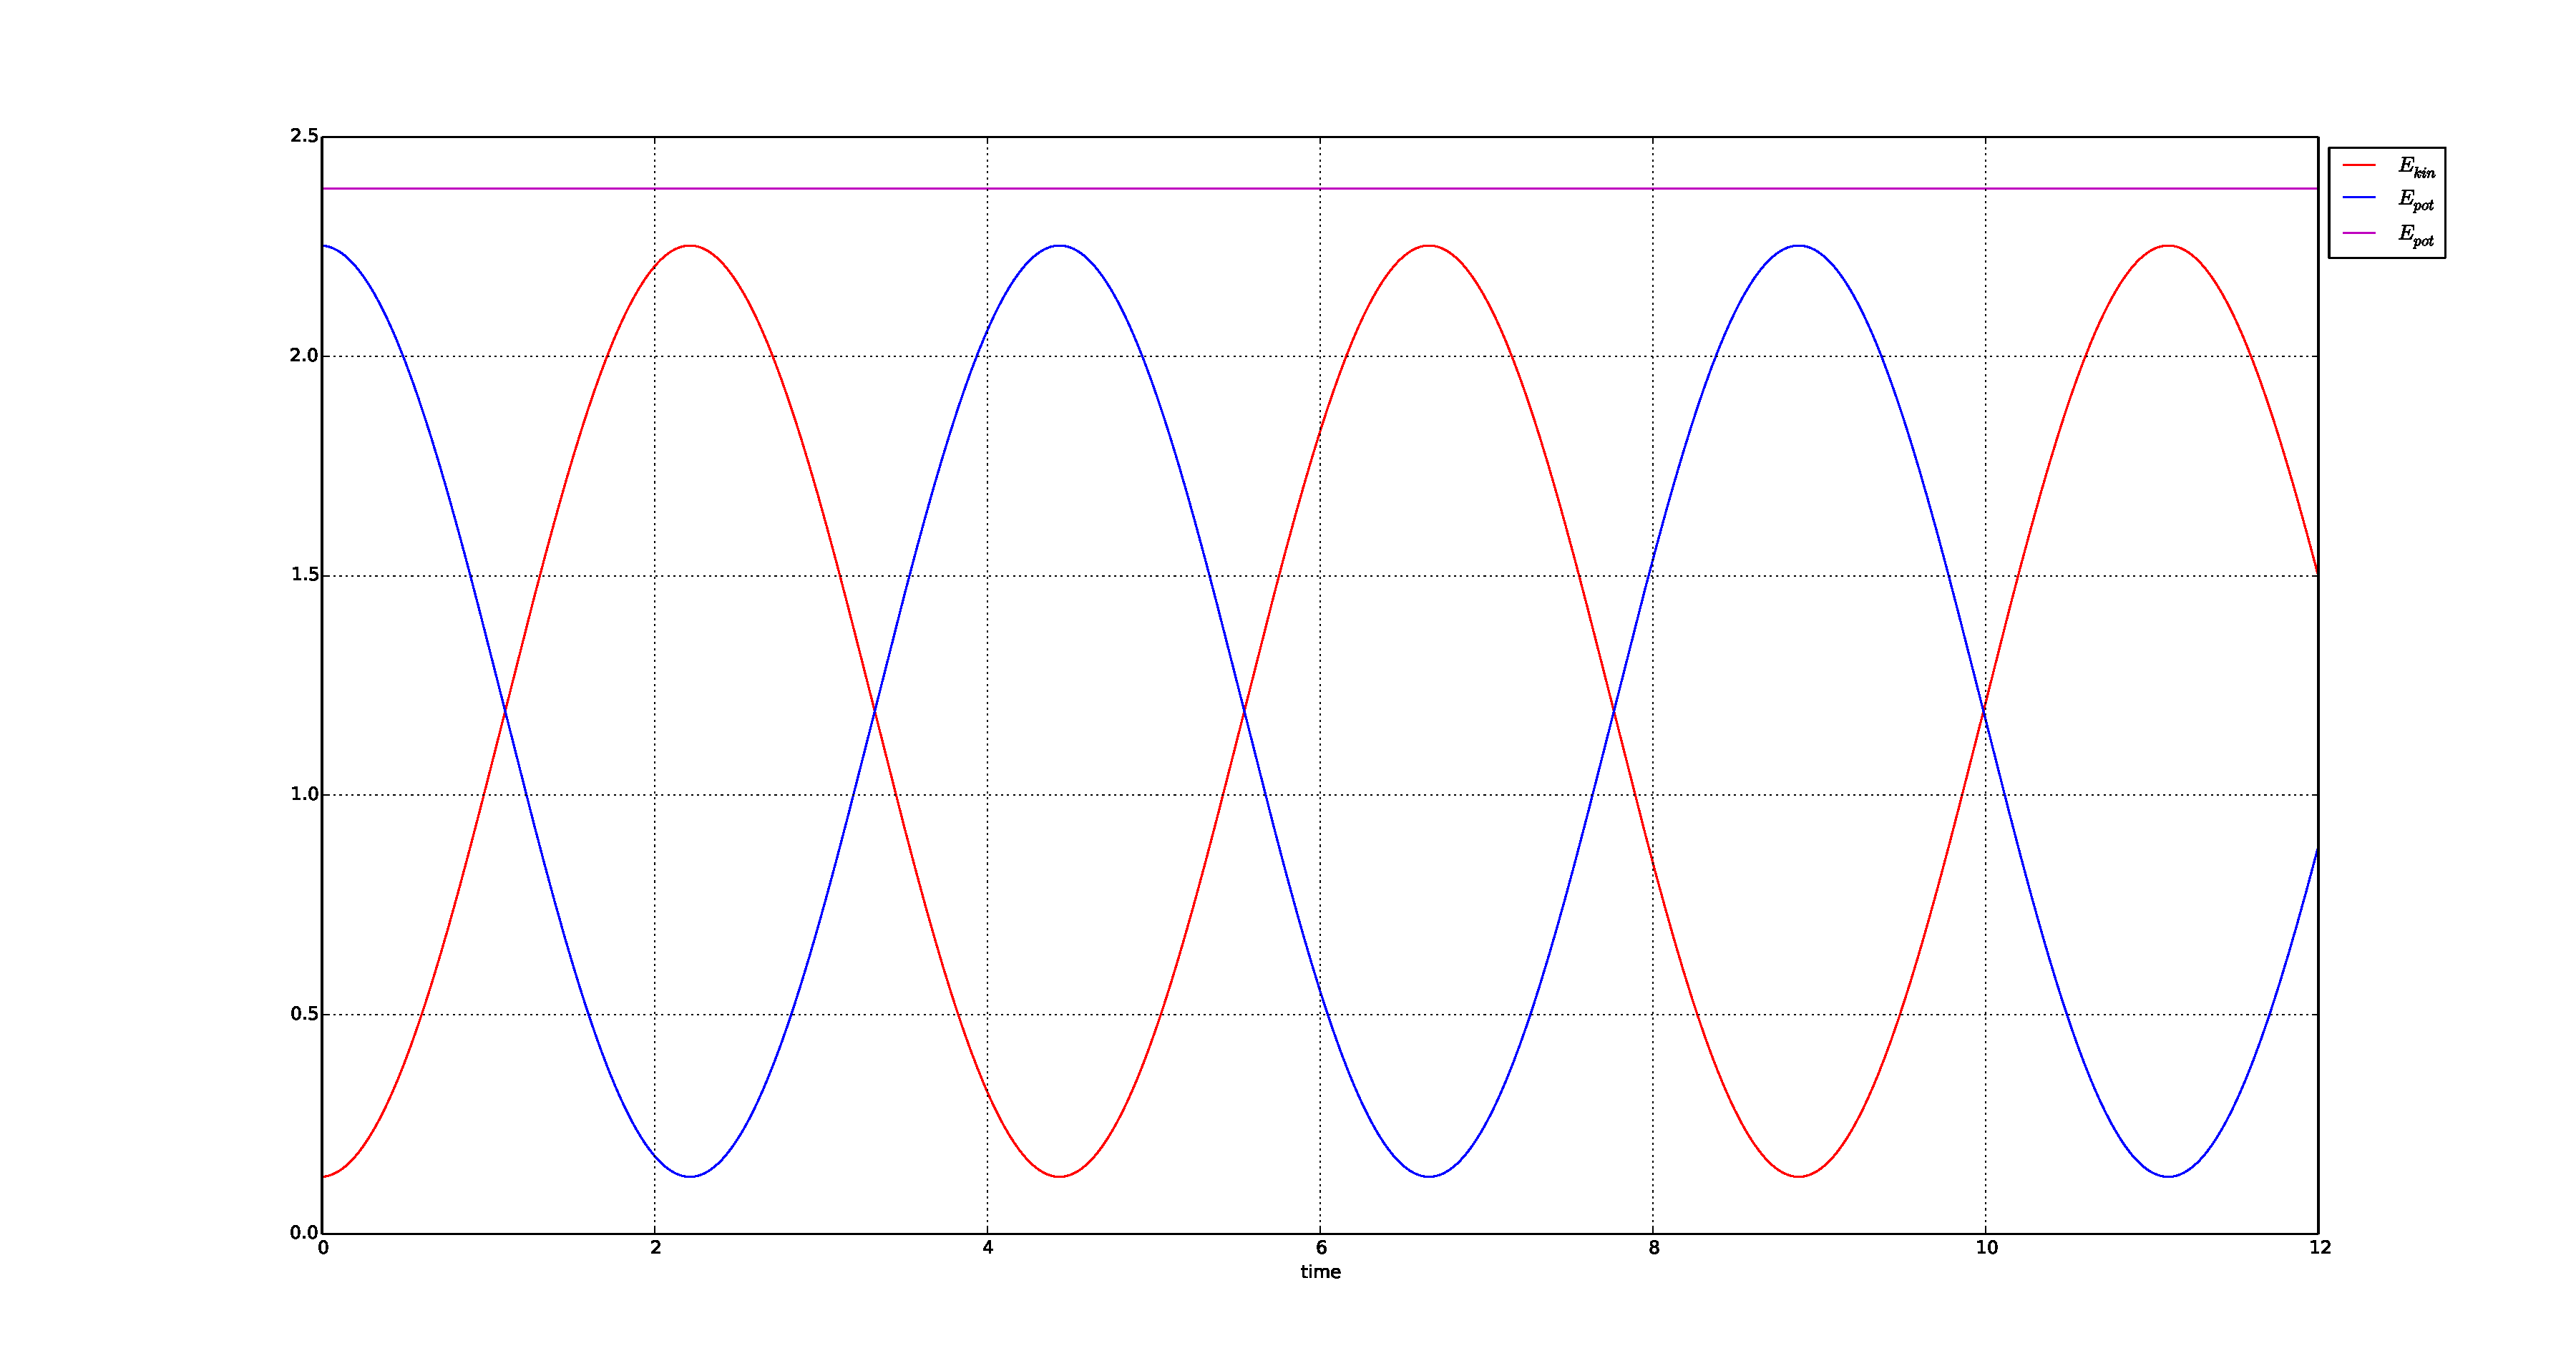
\includegraphics[width=\textwidth]{Figures/harmonic_energy.pdf}
\caption{The energies of the harmonic simulation.}
\label{fig:harmonic_energy}
\end{figure}

\begin{figure}
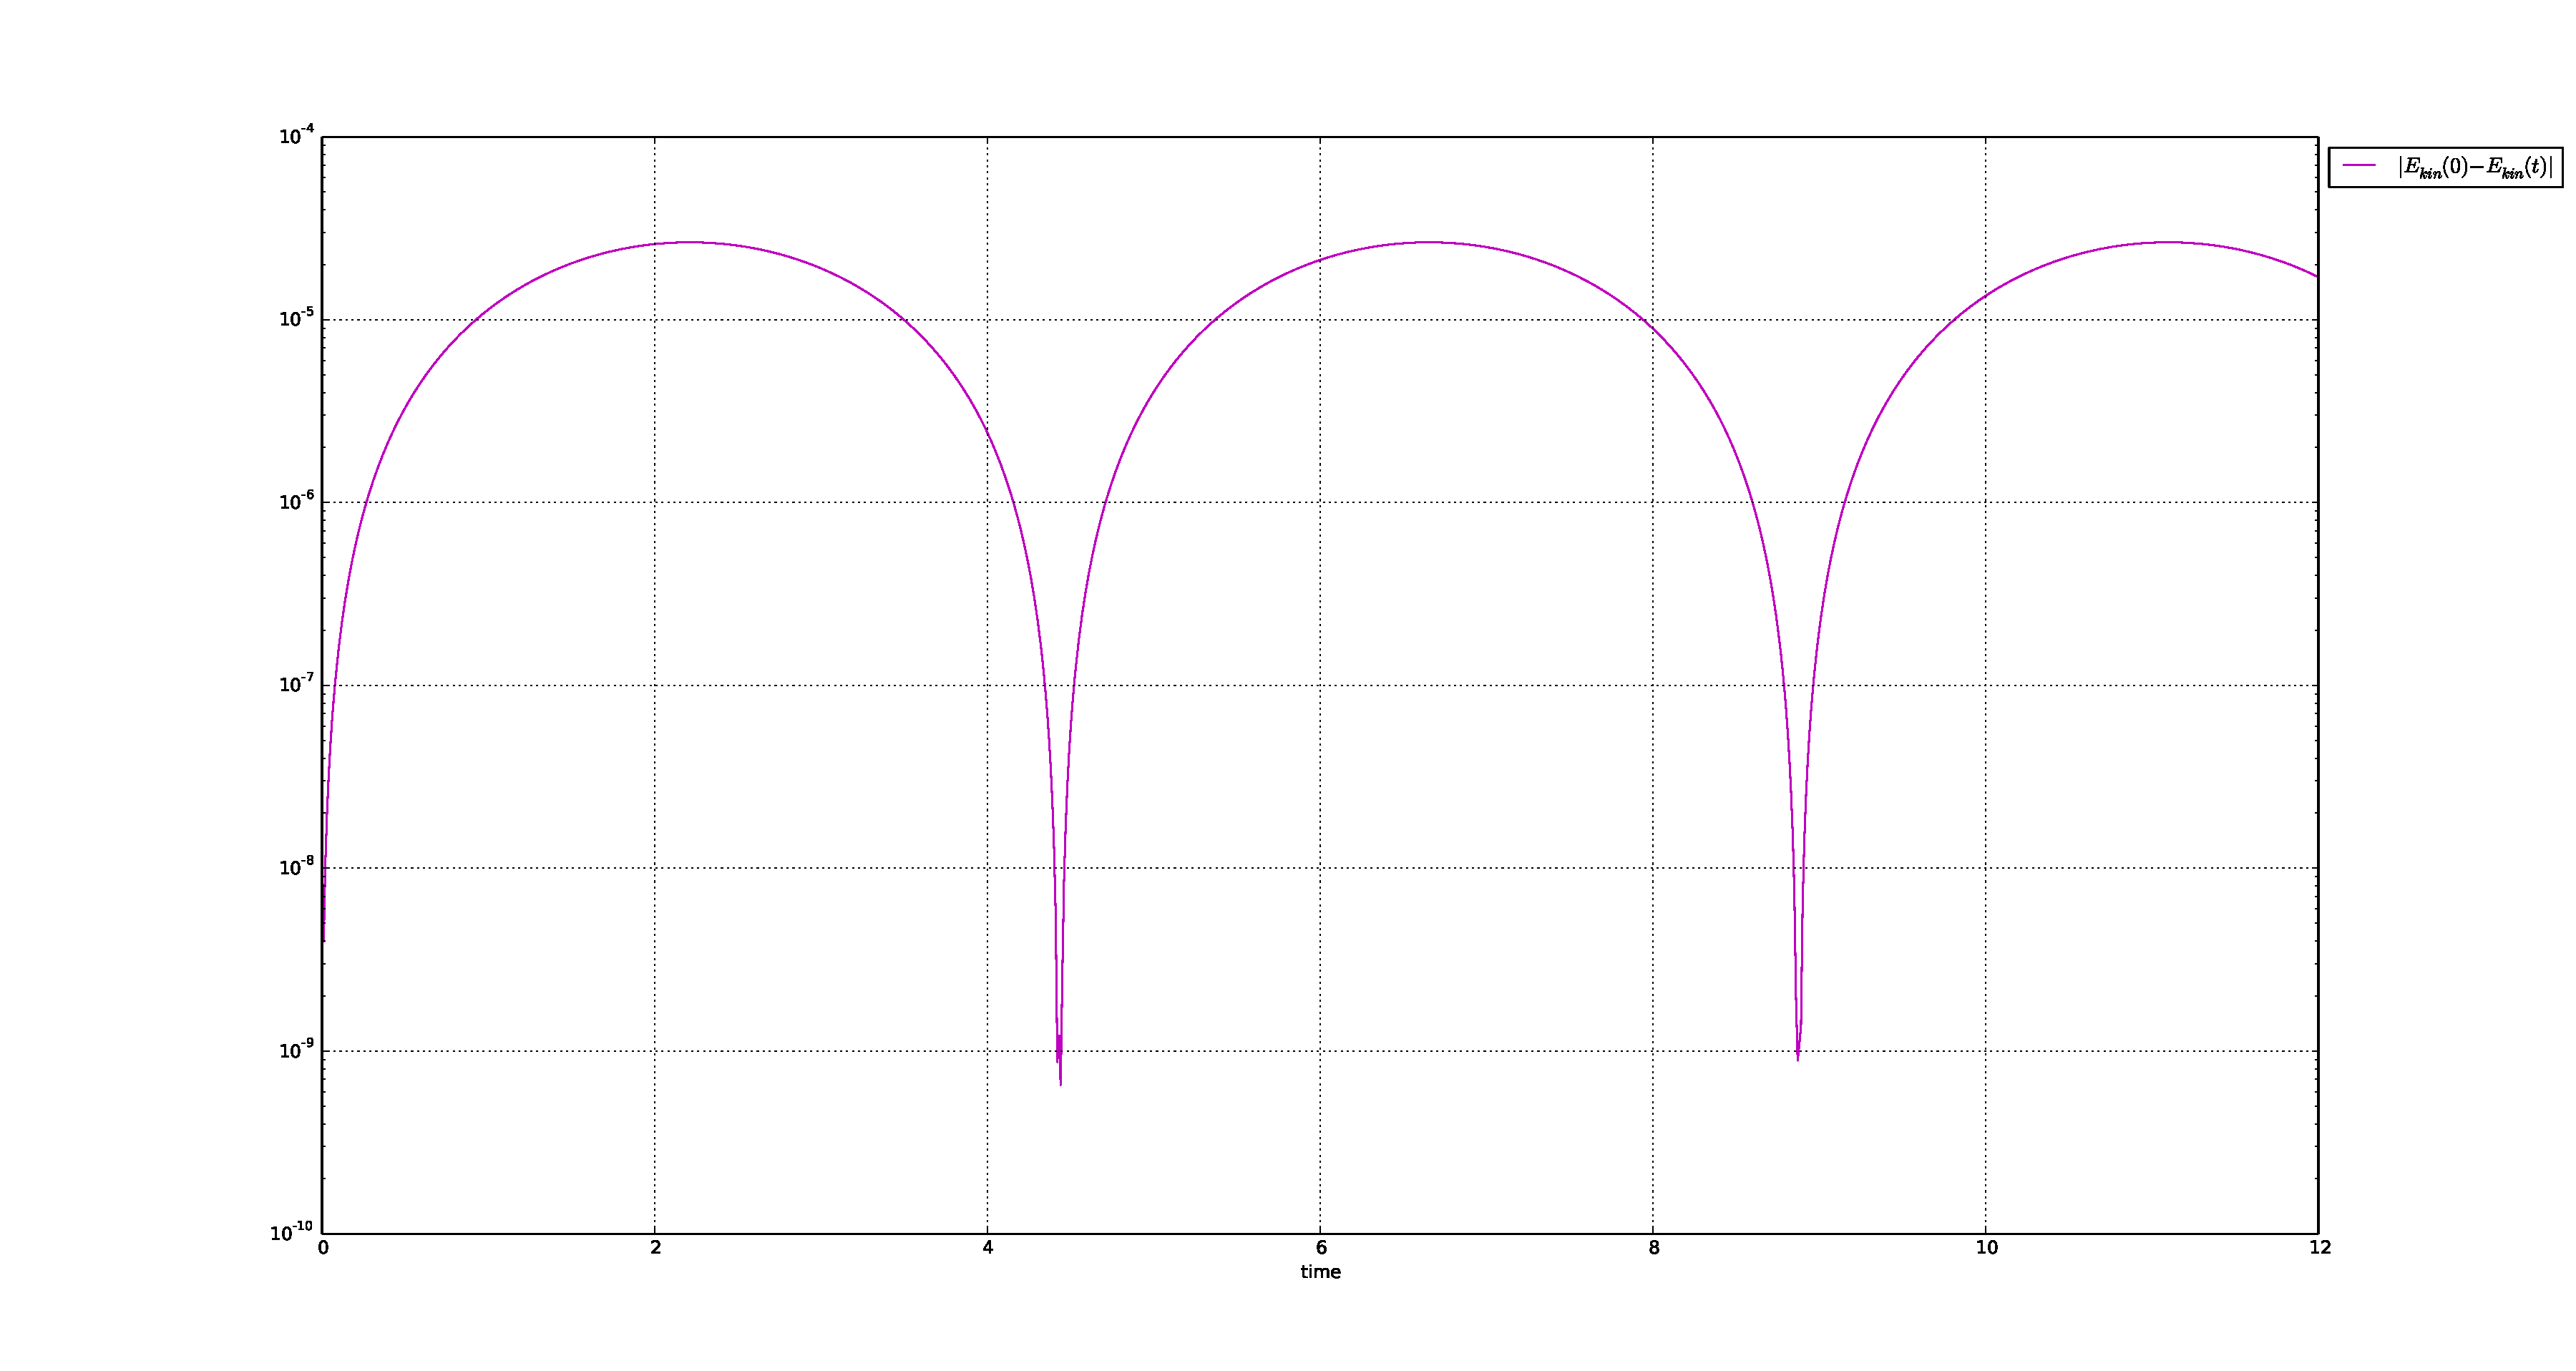
\includegraphics[width=\textwidth]{Figures/harmonic_drift.pdf}
\caption{The drift of the total energies in the harmonic simulation.}
\label{fig:harmonic_drift}
\end{figure}

\begin{figure}[!ht]
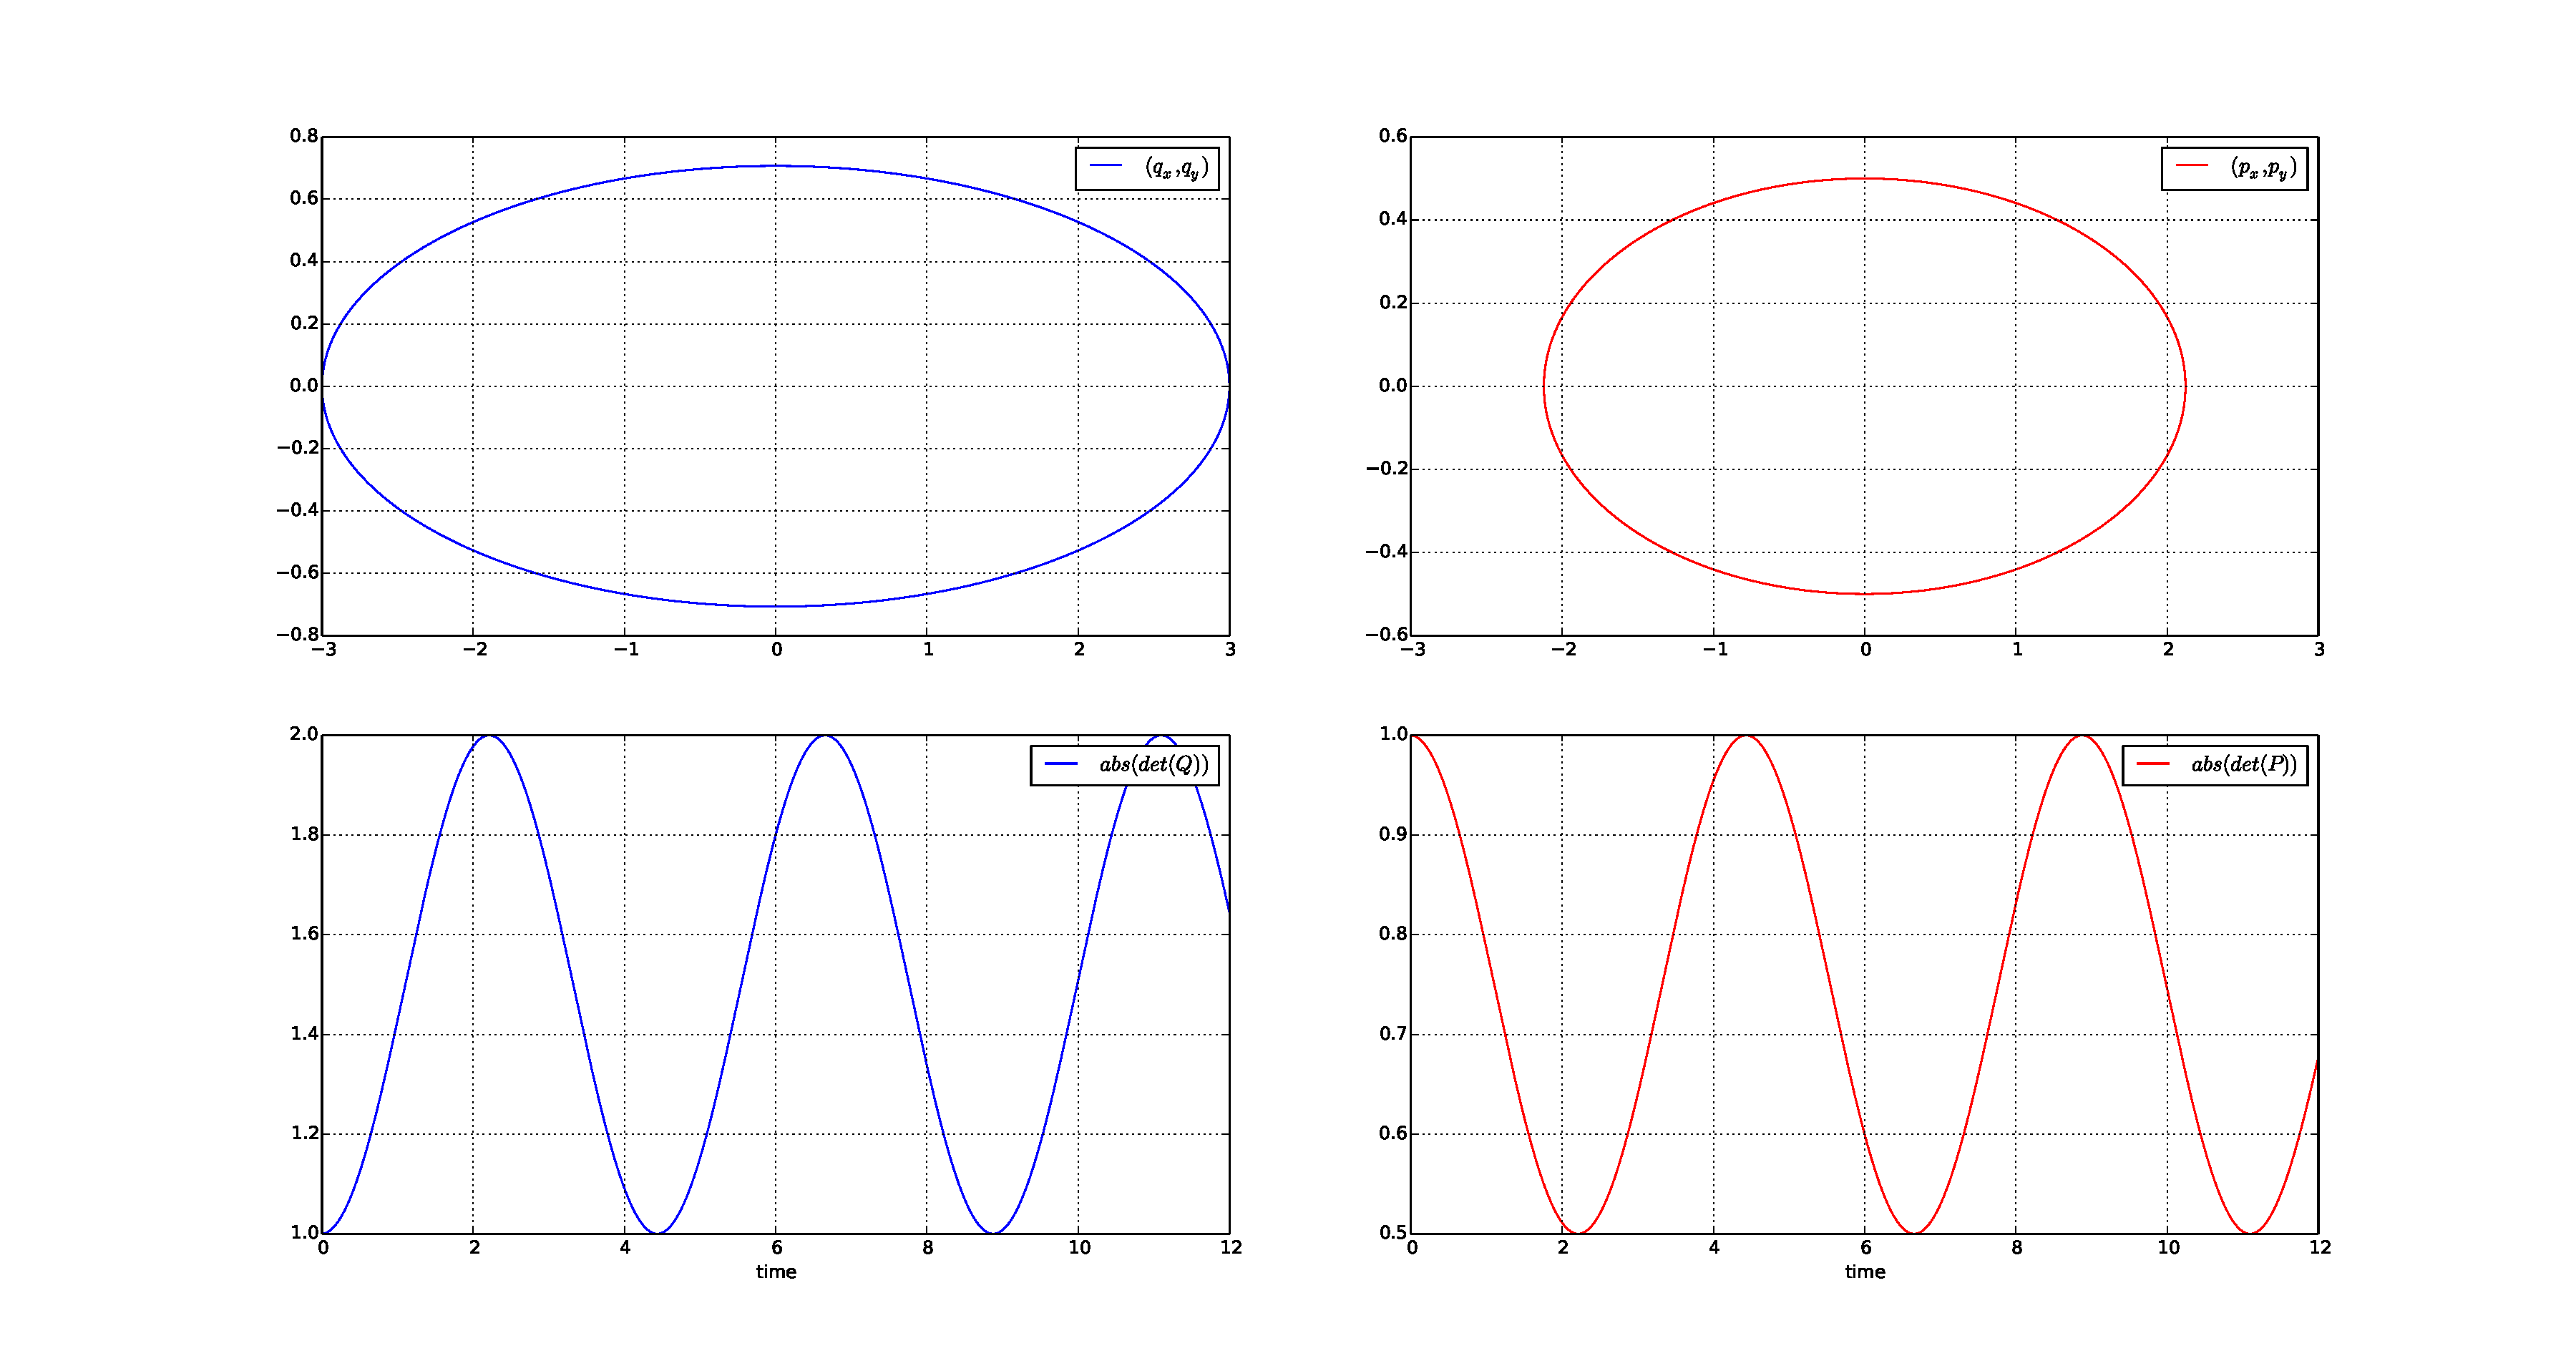
\includegraphics[width=\textwidth]{Figures/harmonic_params.pdf}
\caption{The position and momentum parameters of the harmonic simulation.}
\label{fig:harmonic_params}
\end{figure}
\begin{figure}[!ht]
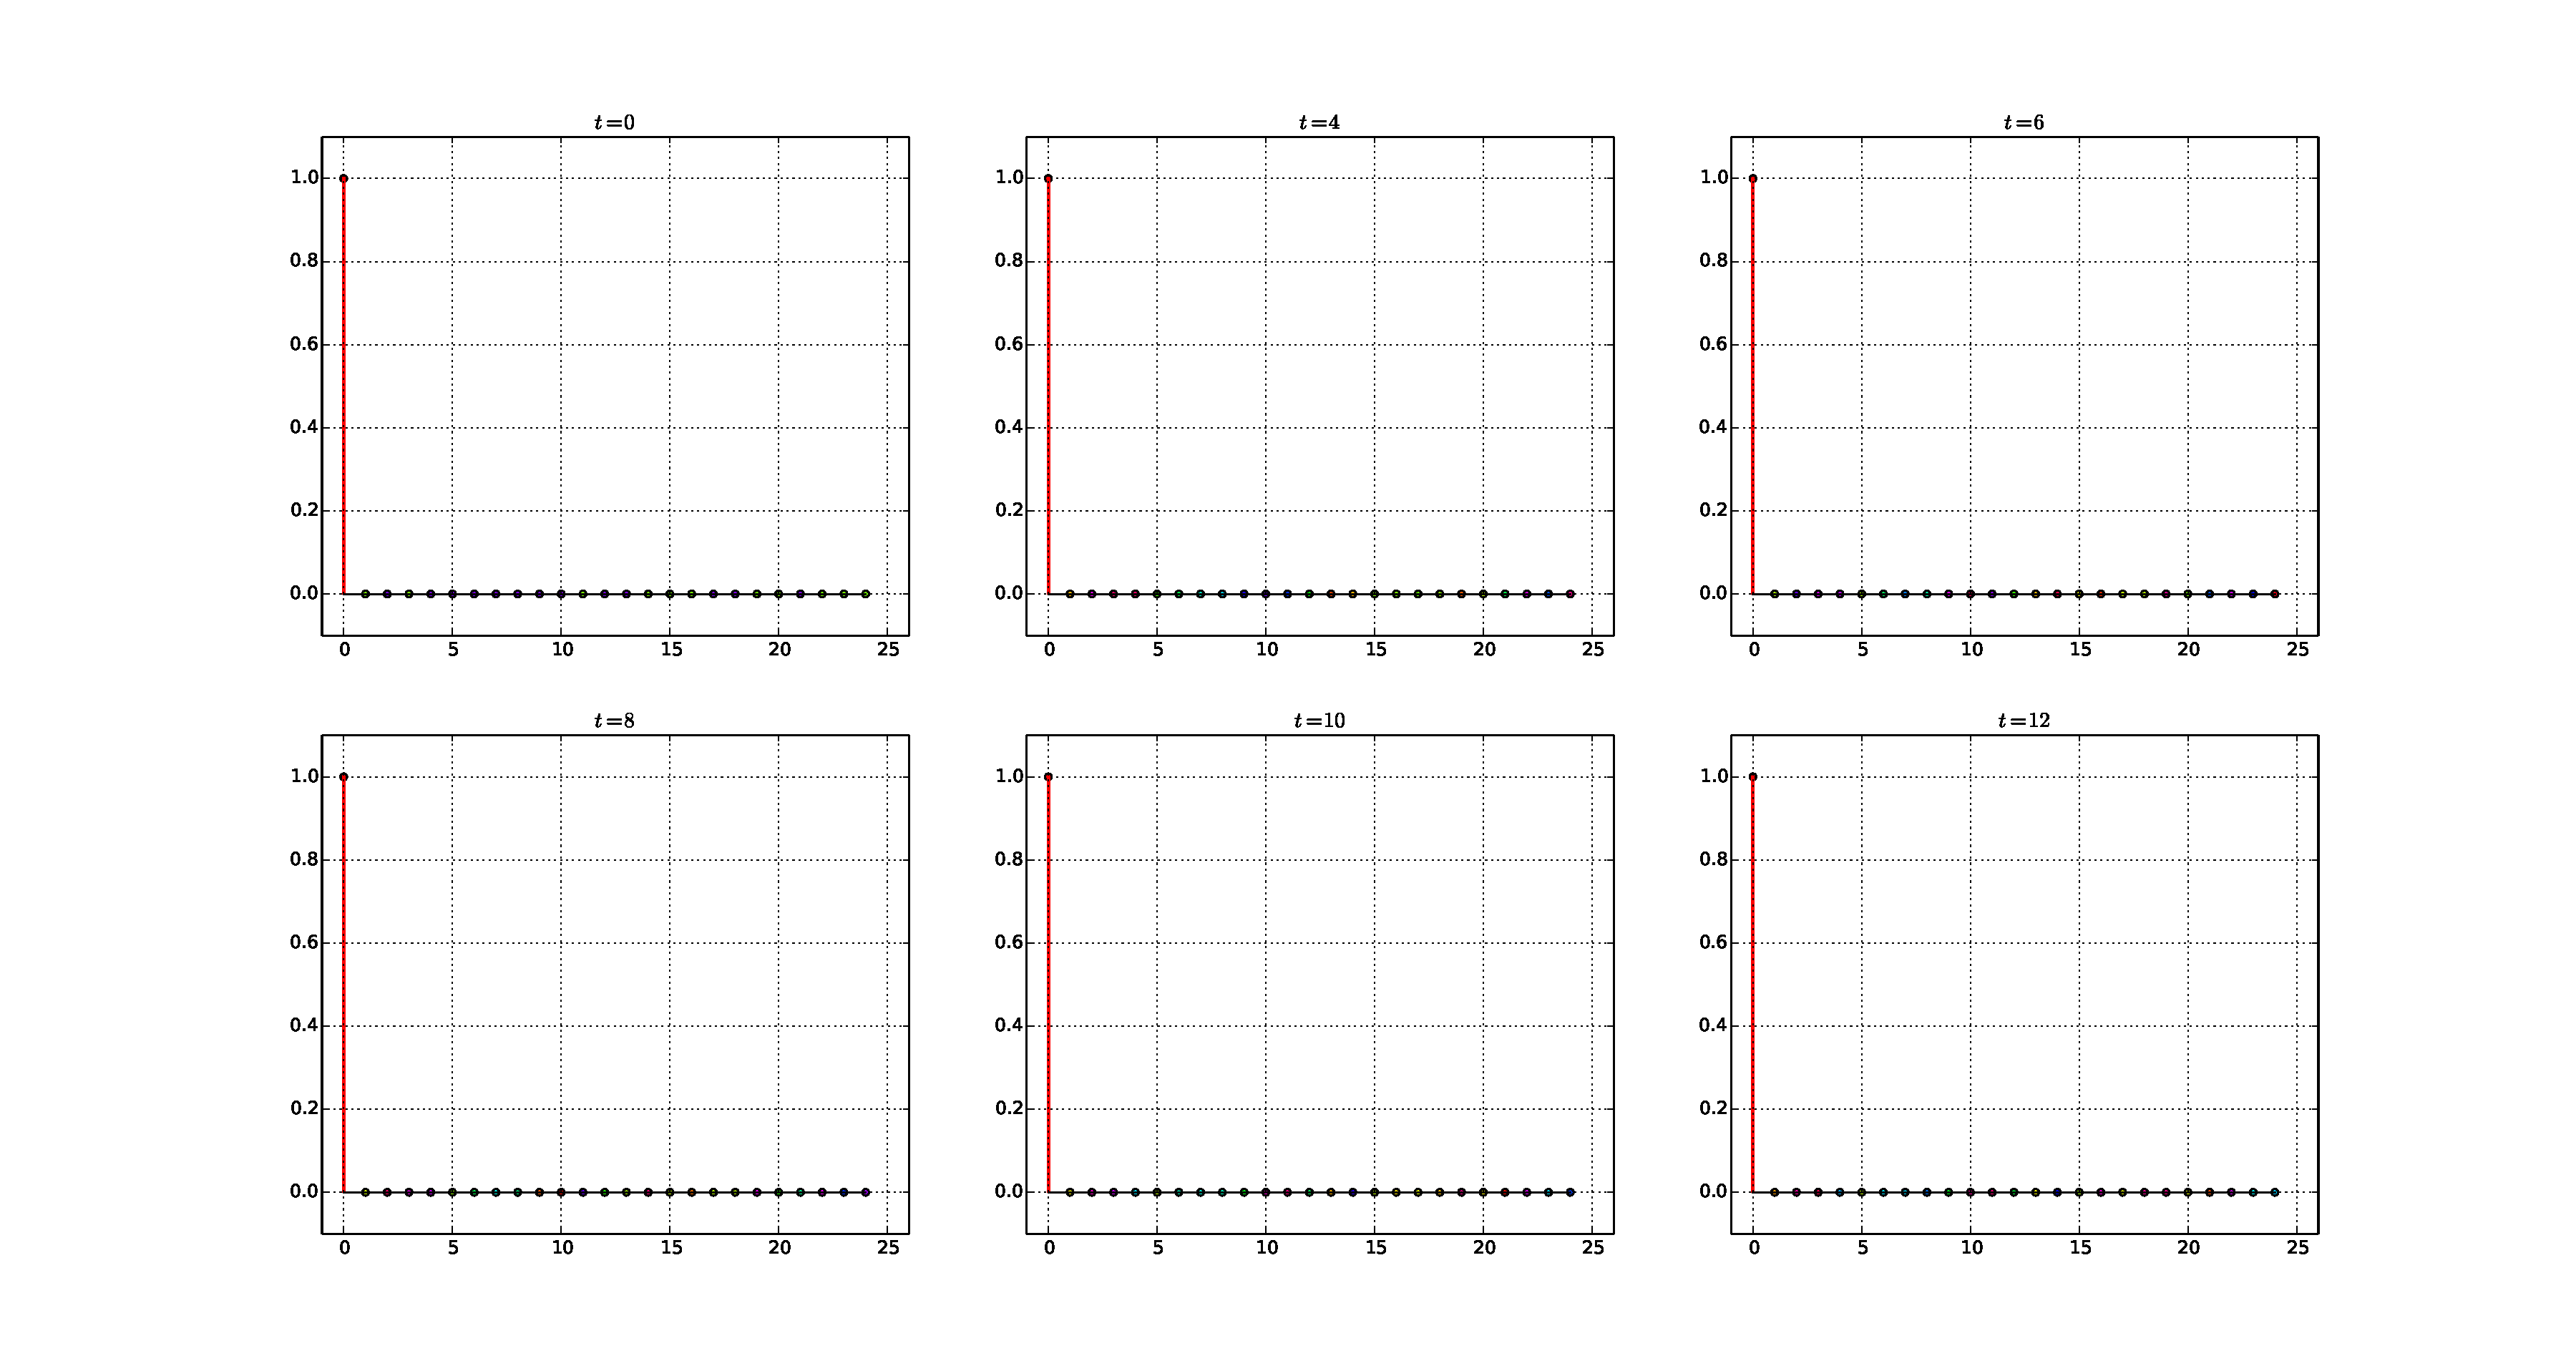
\includegraphics[width=\textwidth]{Figures/harmonic_coeffs.pdf}
\caption{The coefficients of the harmonic simulation.}
\label{fig:harmonic_coeffs}
\end{figure}

\FloatBarrier


\subsection{Anharmonic Oscillator}
This example considers the potential $V: \mathbb{R} \rightarrow \mathbb{R}$ where $V(x) = 1 + x^4$.

A Gaussian Hagedorn wavepacket with $128$ cubic shape basis functions with the following initial parameters:
\begin{center}
 \begin{tabular}{|c c c c c c|} 
 \hline
 q & p & Q & P & S & $\varepsilon$\\ [0.5ex] 
 \hline
 0 & 1 & 1 & i & 0 & 0.1\\ 
 \hline
\end{tabular}
\end{center}
is propagated using the Hagedorn propagator with $dt = 0.01$ up to $T = 6$.

Figure \ref{fig:anharmonic_drift} shows quite neat conservation of energy until the second reflection at which point the simulation seems to break down. This observation as well as the other plots are consistent with the \texttt{WaveBlocksND} implementation of the same example which serves as an indicator that the implementation is also correct in the anharmonic part.

\begin{figure}
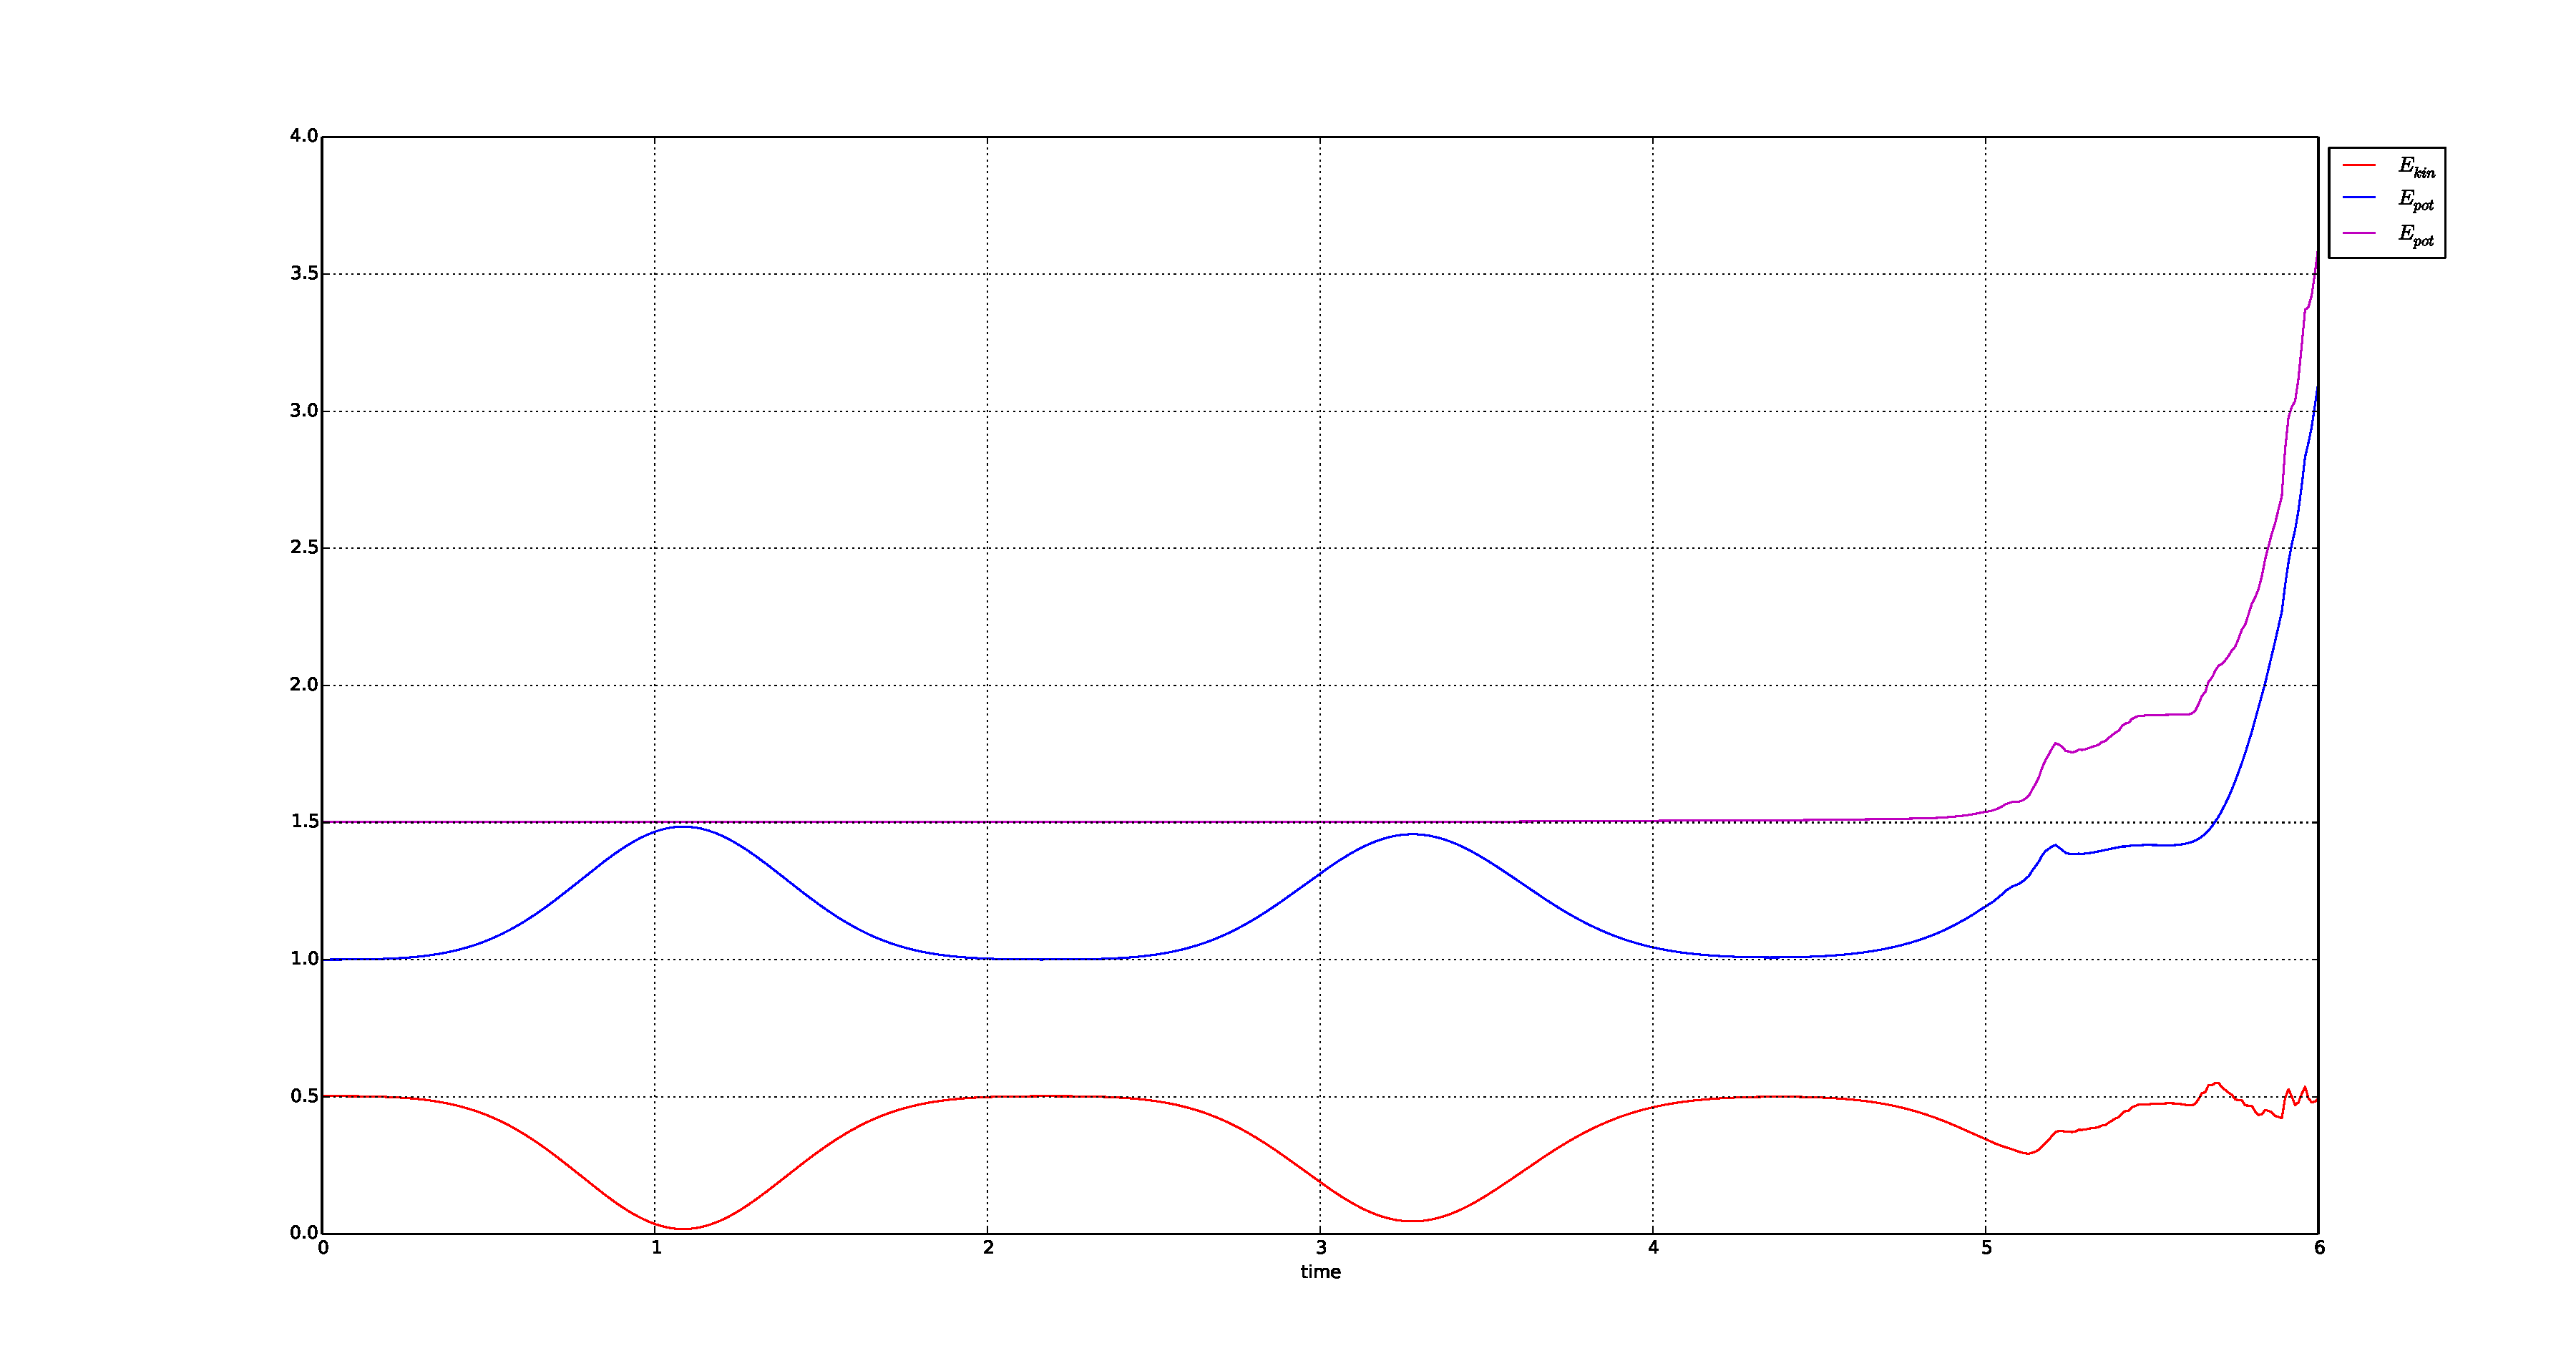
\includegraphics[width=\textwidth]{Figures/anharm_energy.pdf}
\caption{The energies of the anharmonic simulation.}
\label{fig:anharmonic_energy}
\end{figure}

\begin{figure}
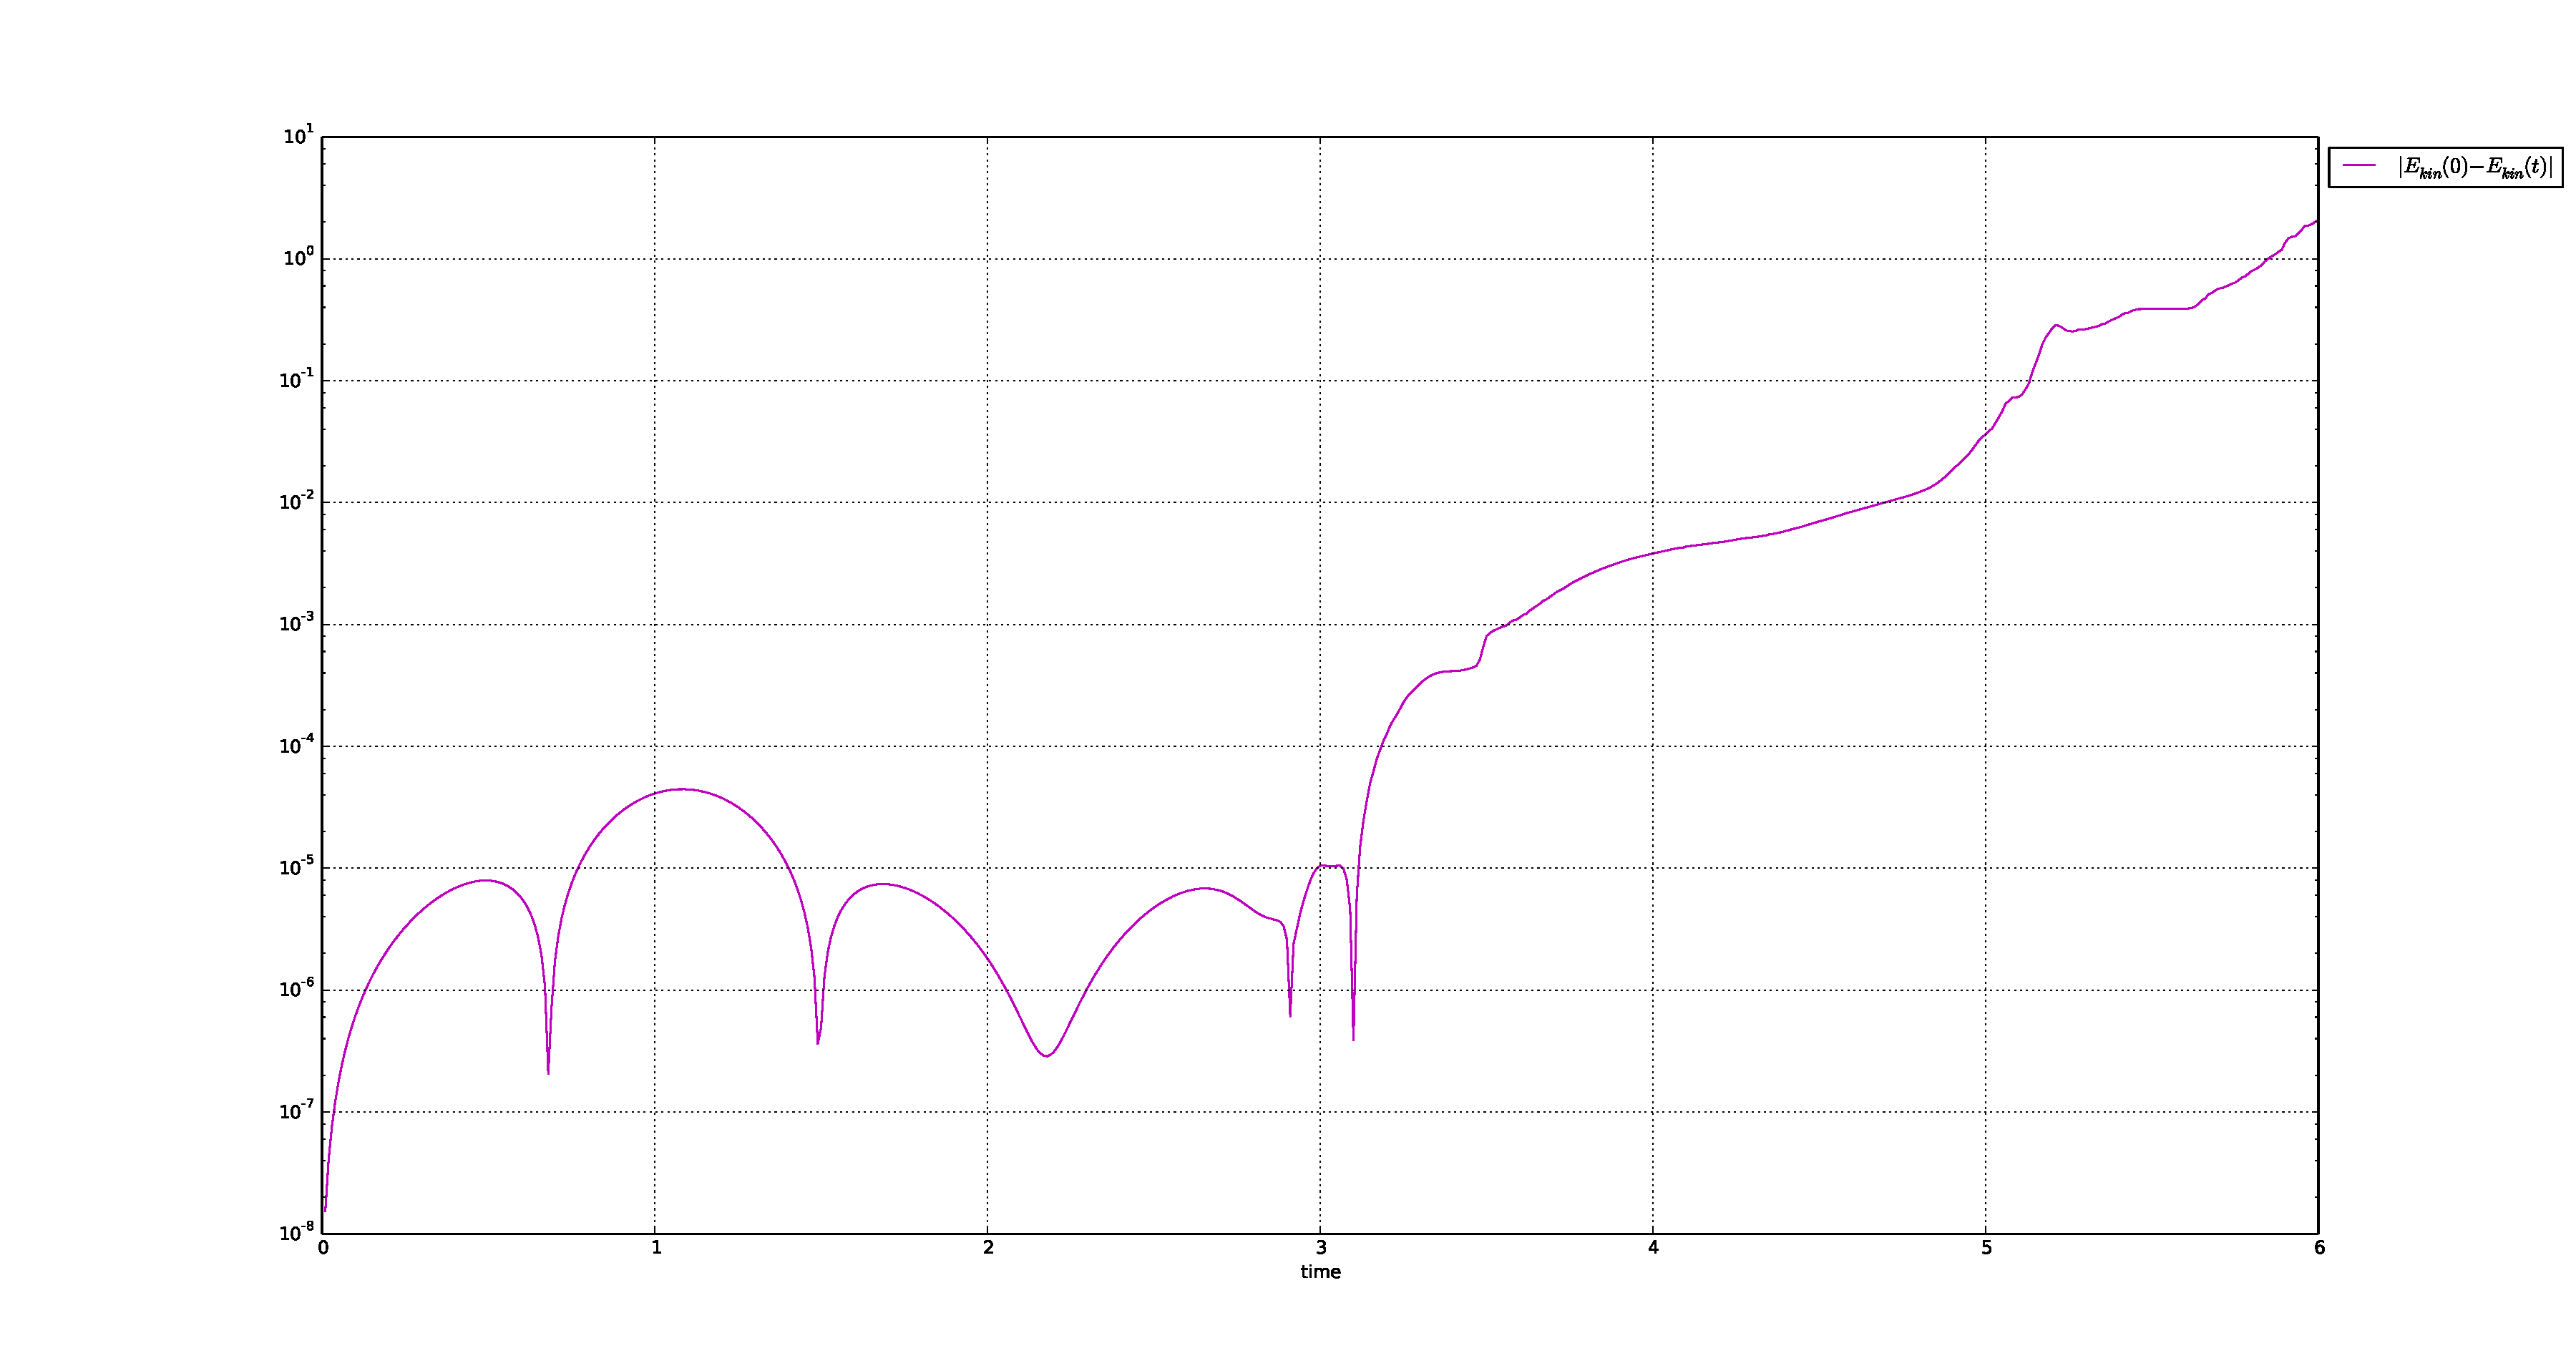
\includegraphics[width=\textwidth]{Figures/anharmonic_drift.pdf}
\caption{The drift of the total energies in the anharmonic simulation.}
\label{fig:anharmonic_drift}
\end{figure}

\begin{figure}
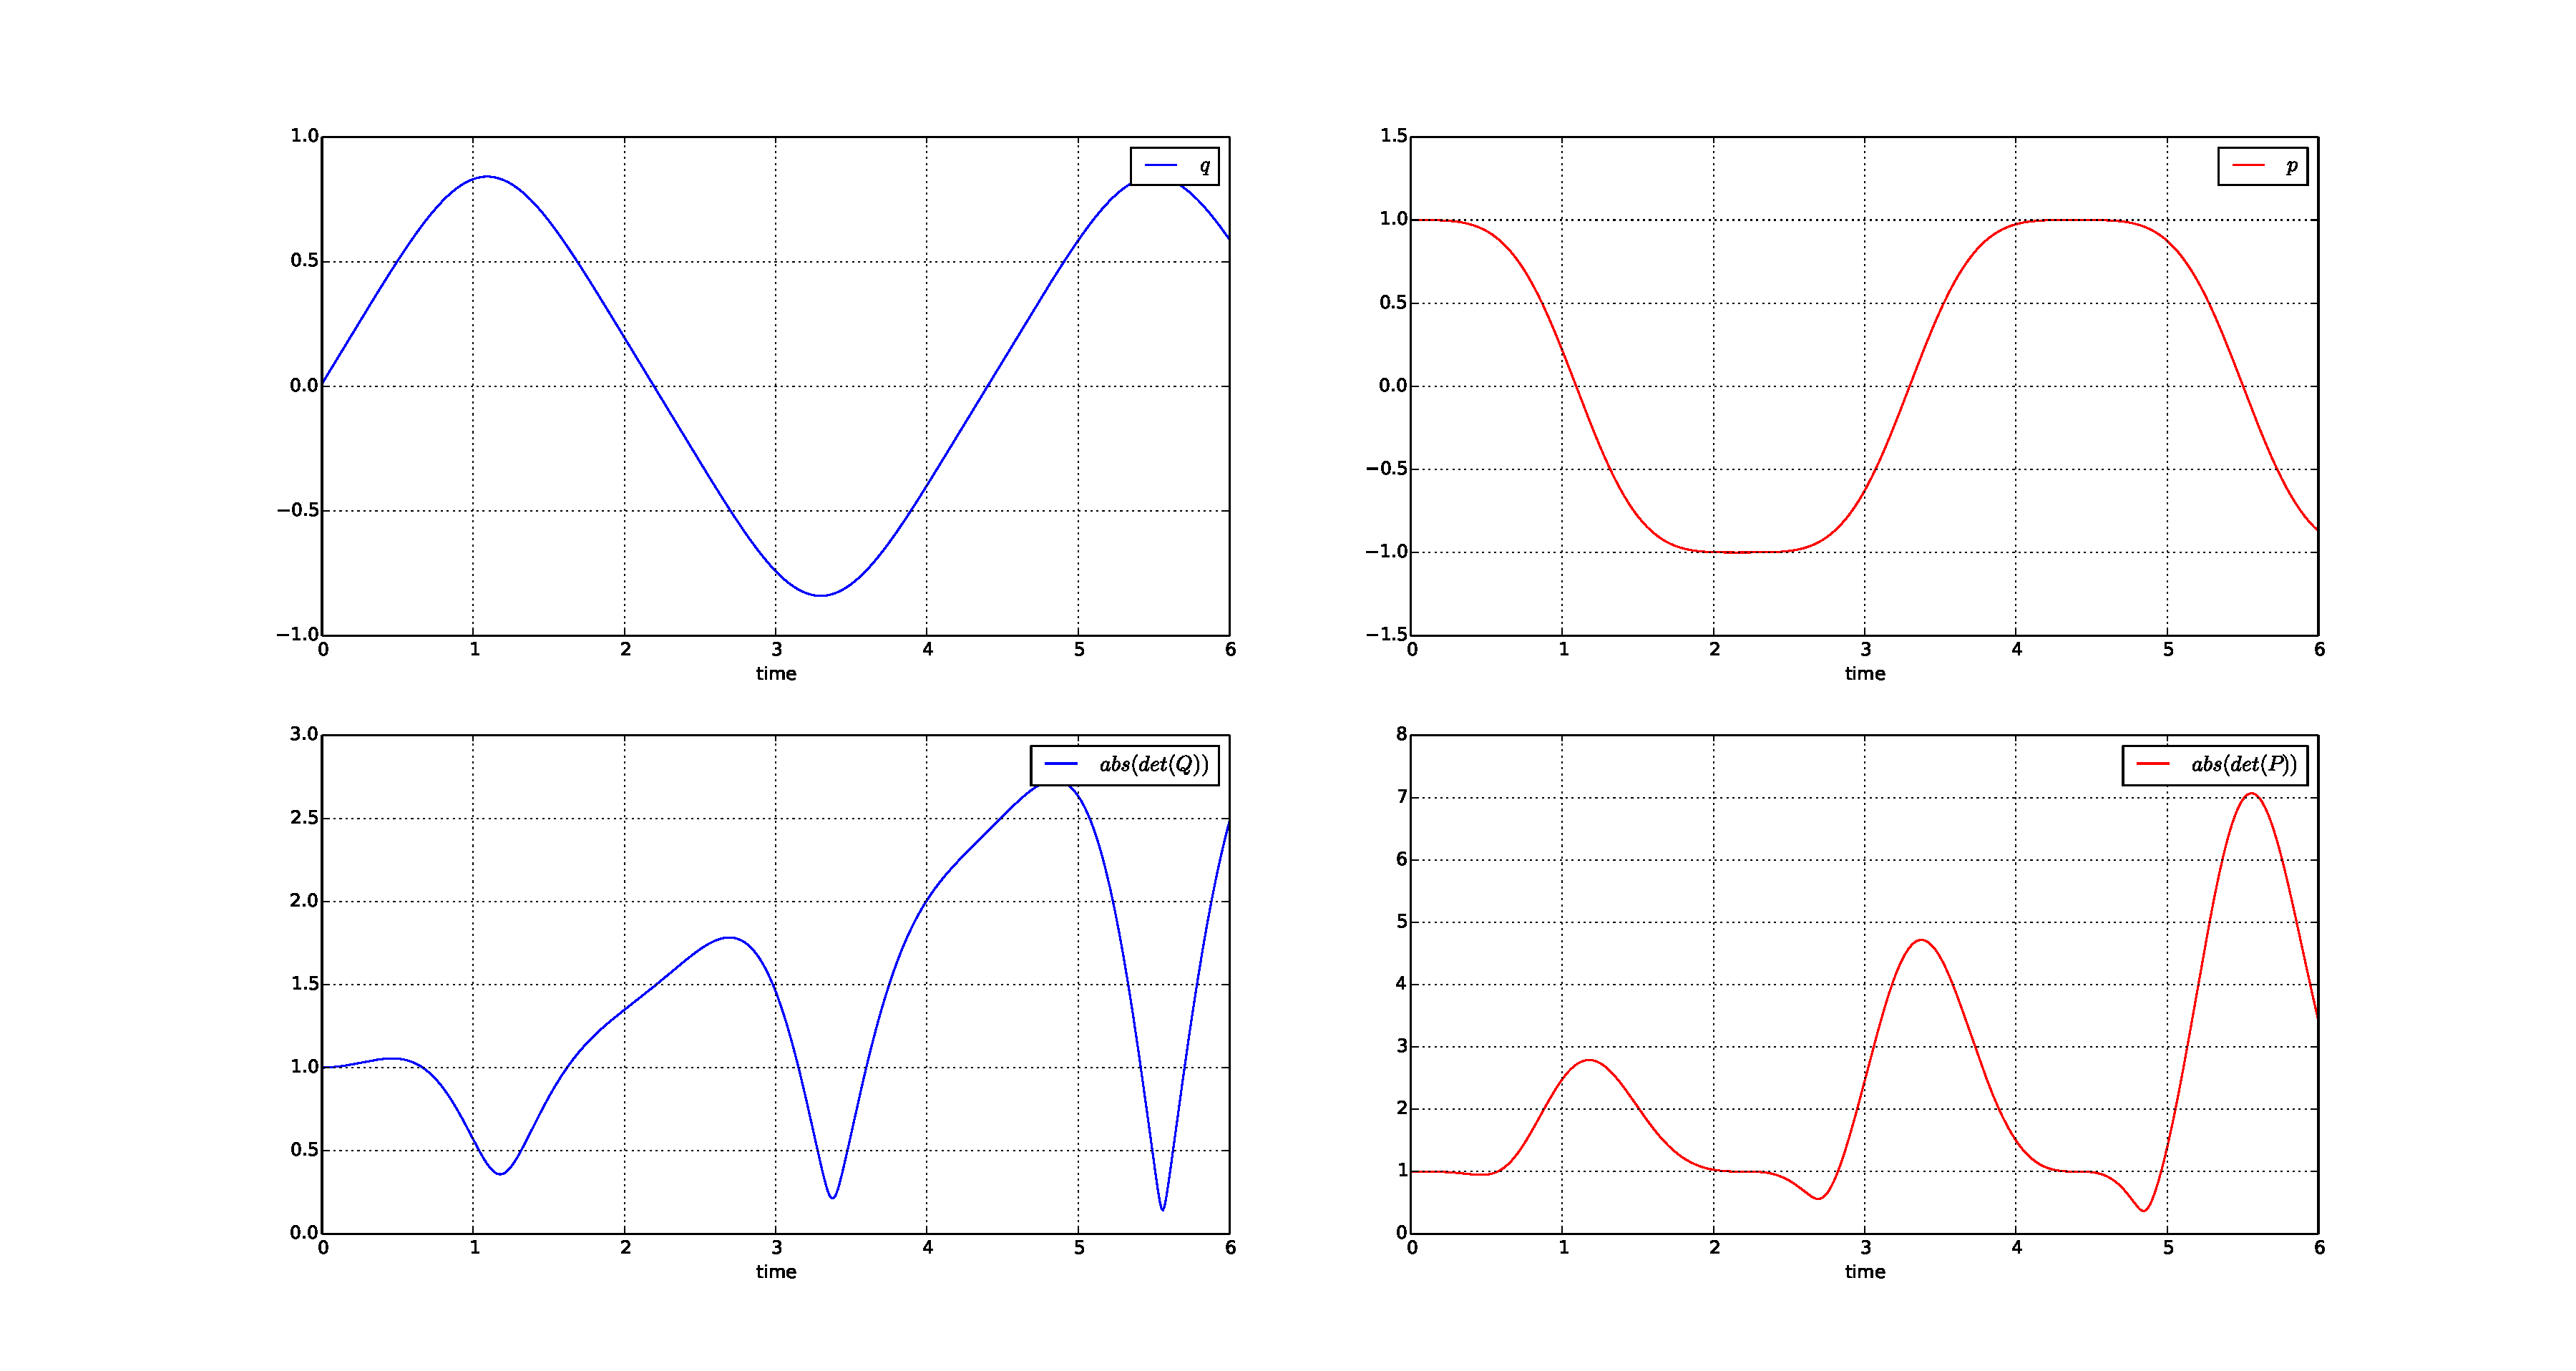
\includegraphics[width=\textwidth]{Figures/anharm_params.pdf}
\caption{The position and momentum parameters of the harmonic simulation.}
\end{figure}
\begin{figure}
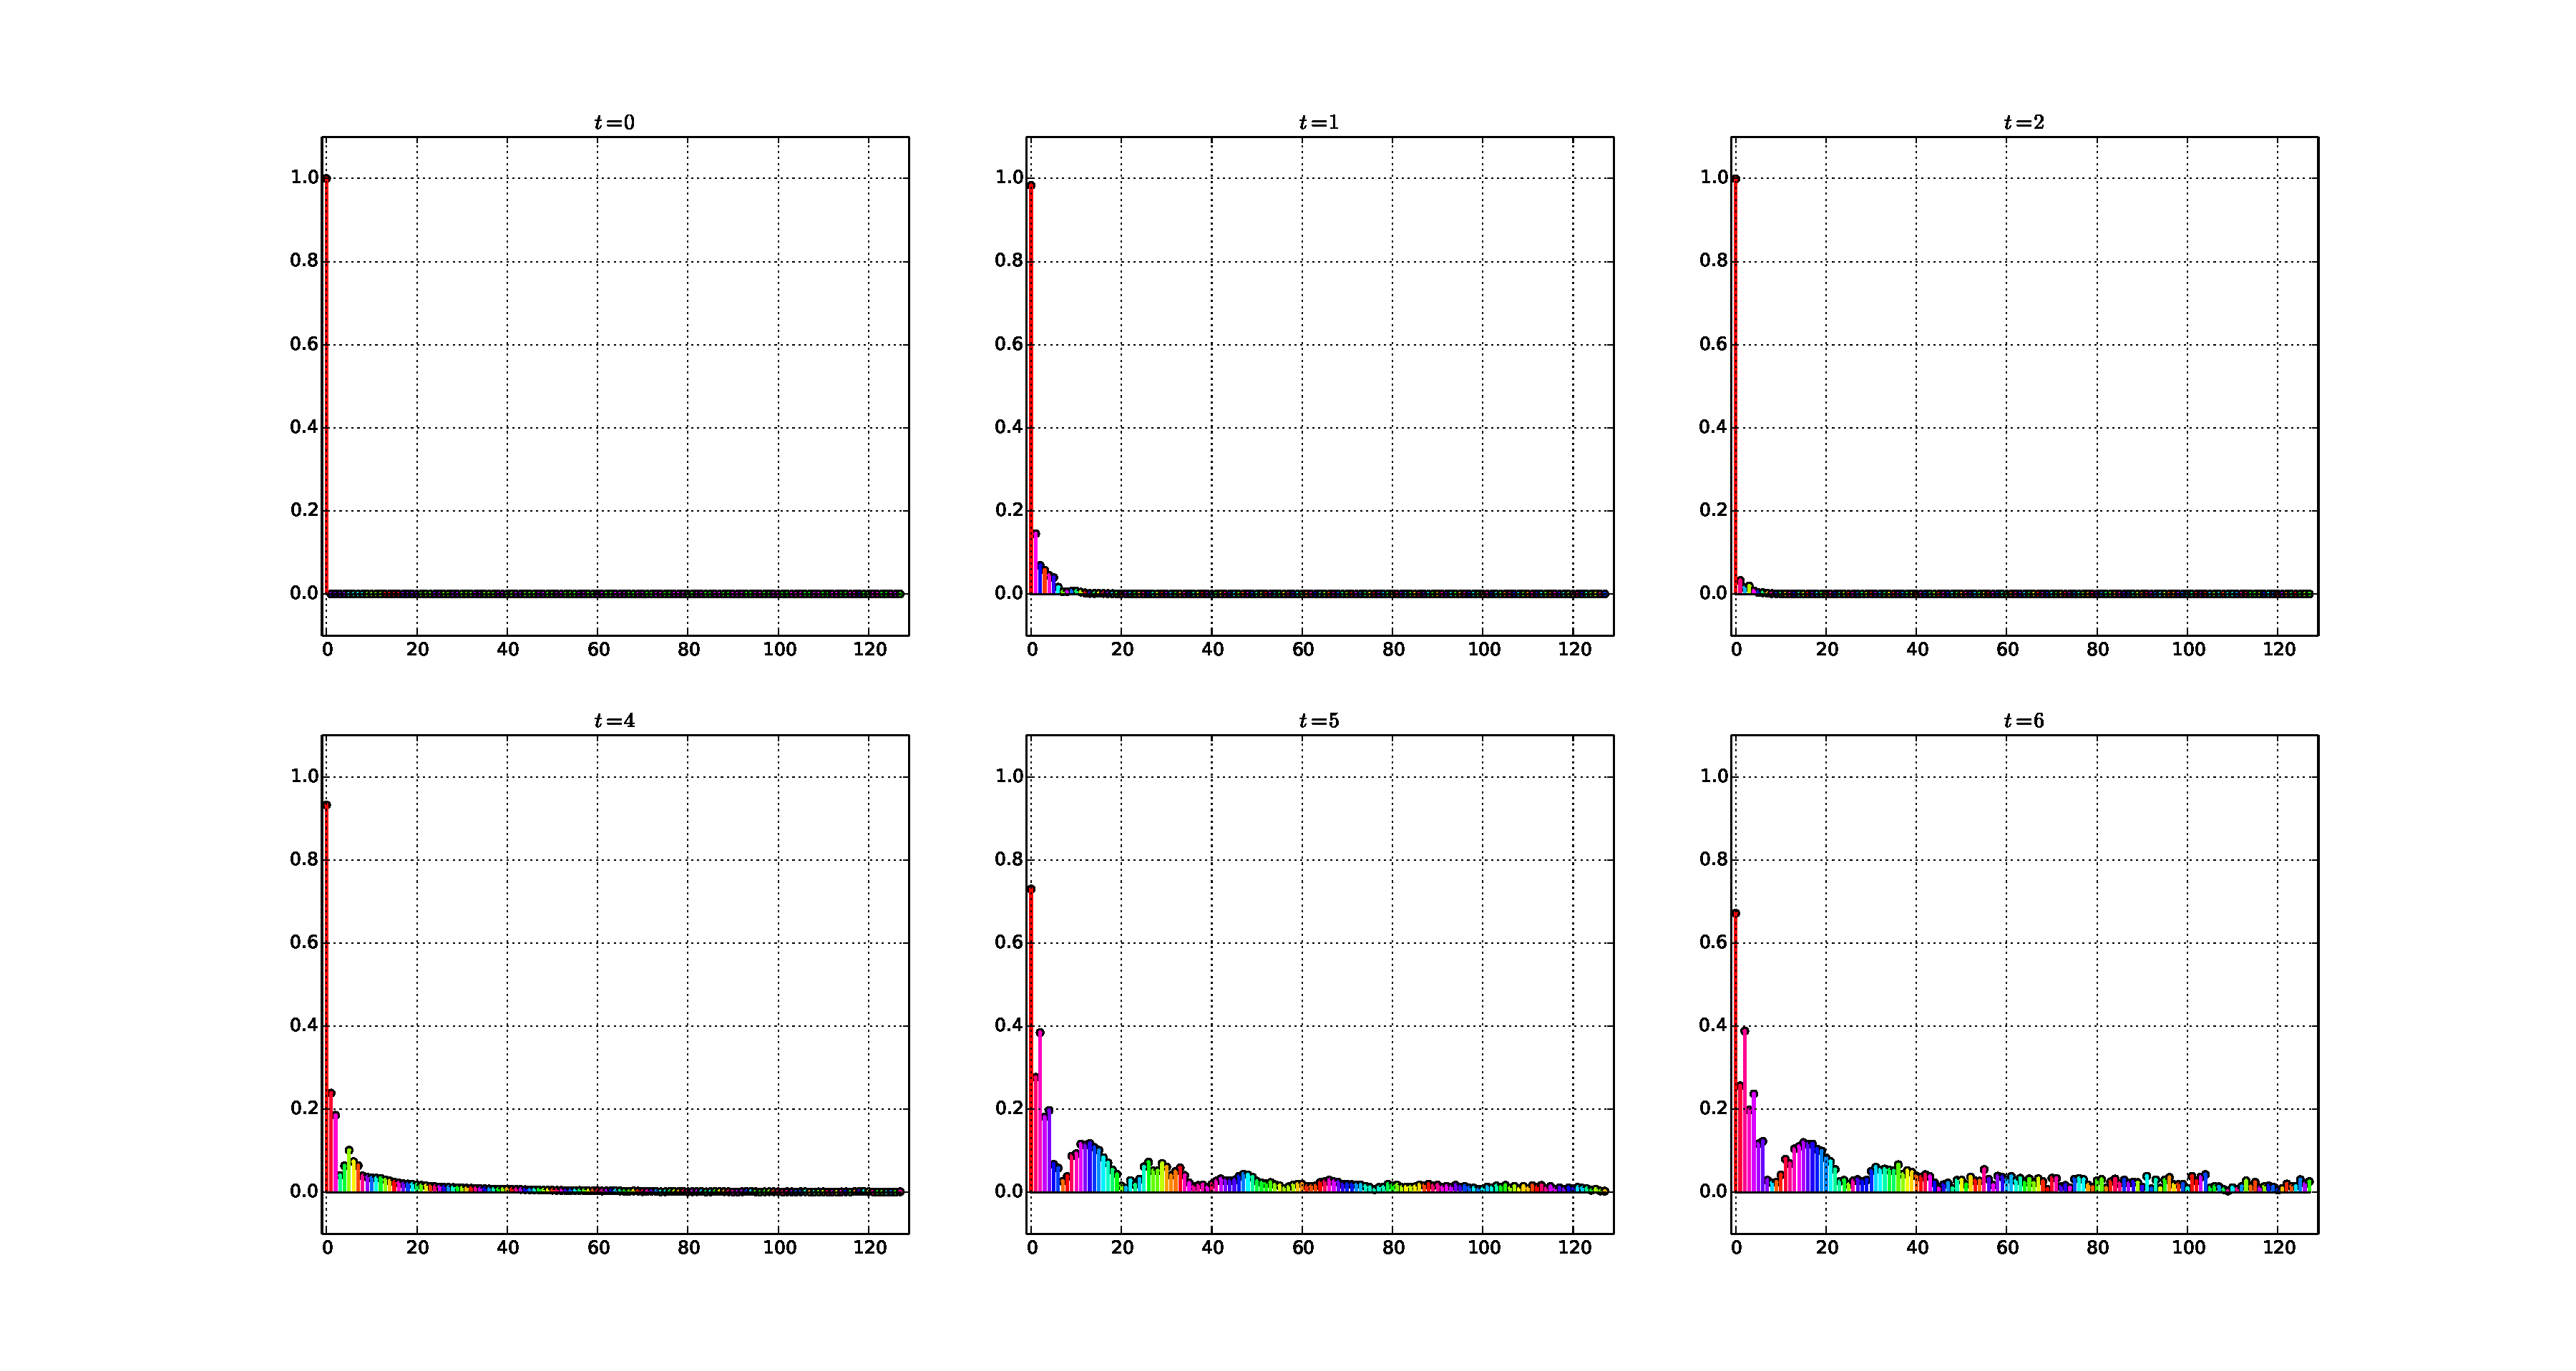
\includegraphics[width=\textwidth]{Figures/anharm_coeffs.pdf}
\caption{The coefficients of the harmonic simulation.}
\end{figure}
\FloatBarrier

\subsection{Conclusion}
Both simulations were consistent with the \texttt{WaveBlocksND} implementation which gives confidence that the implementation is correct for $N=1$.

\section{1D Tunneling}
I attempt to recompute the simulation in \cite{GHJ_tunneling_spawning} as an application of the \texttt{C++} framework.
\subsection{Setup}
Consider the scalar potential $V: \mathbb{R} \rightarrow \mathbb{R}$ with $V(x) = { \sigma \over \cosh(x/a)^2 }$, where $\sigma = 100 {\text{kJ} \over \text{mol}} = 0.038088 \text{ Eh}$ and $a = 0.5\text{ \r{A}} = 0.944858 \text{ alu}$ (as in Figure \ref{fig:tunneling_pot}). 
\begin{figure}
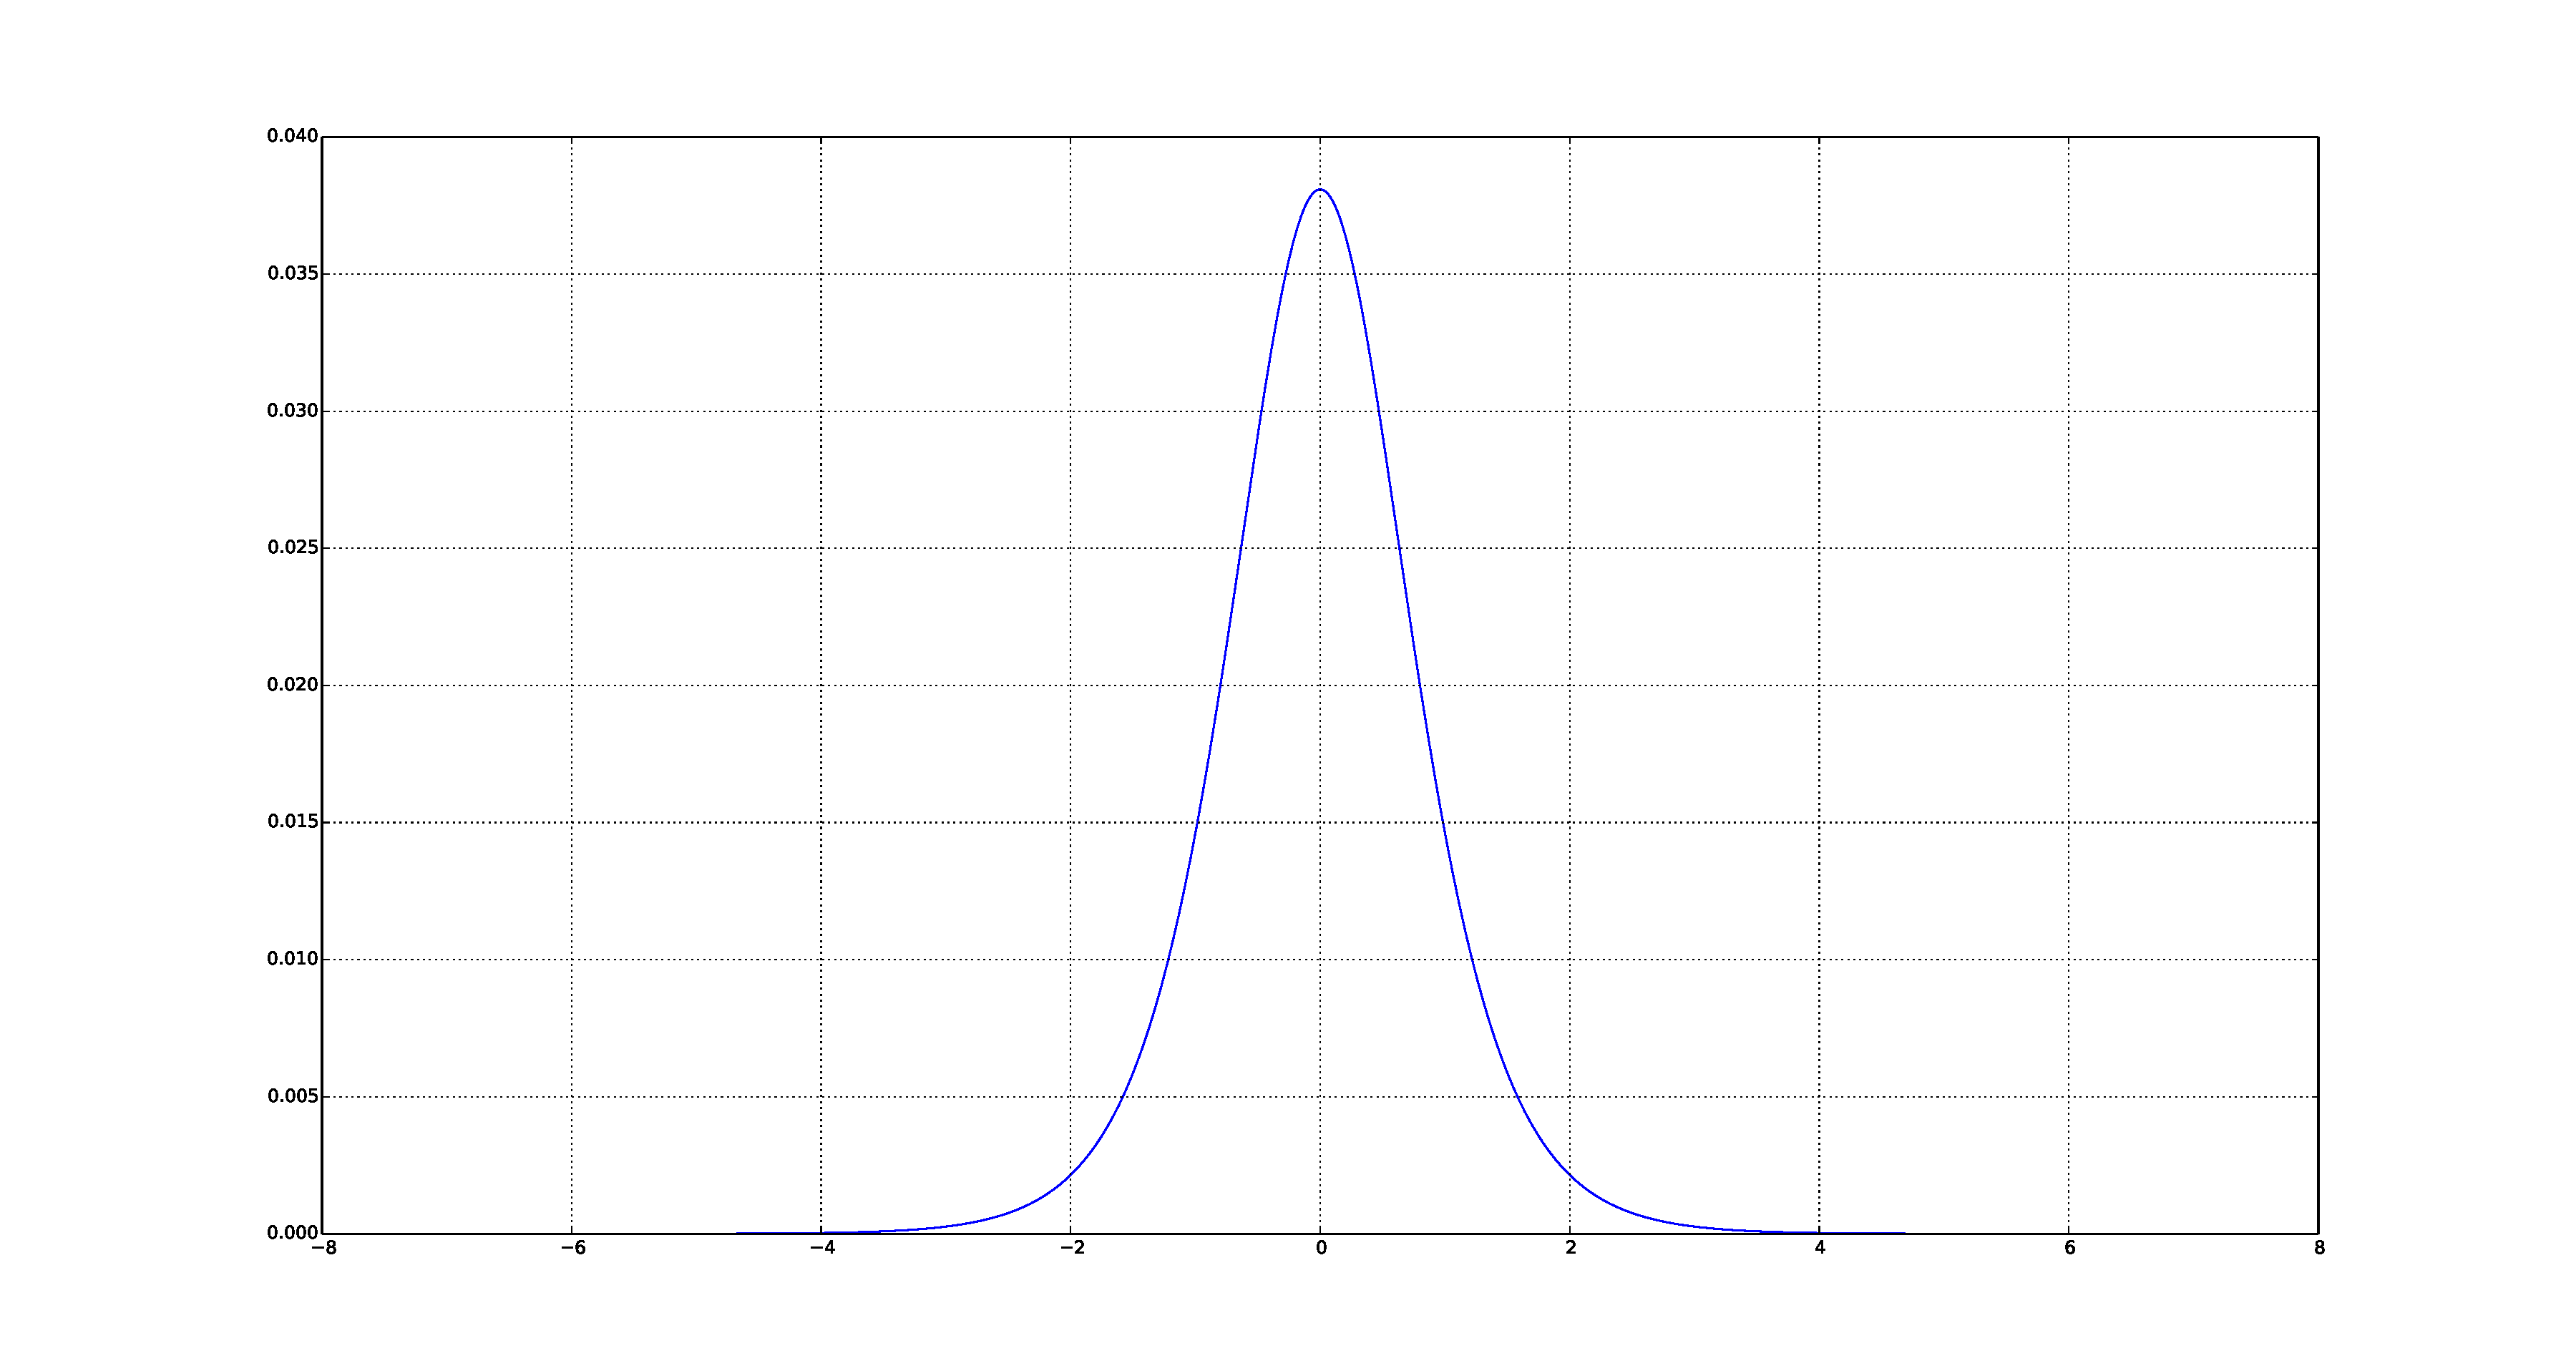
\includegraphics[width=\textwidth]{Figures/tunneling_pot.pdf}
\caption{Potential of the Tunneling Simulation}
\label{fig:tunneling_pot}
\end{figure}
\FloatBarrier

A Gaussian Hagedorn wavepacket with $512$ cubic shape basis functions with the following initial parameters:
\begin{center}
 \begin{tabular}{|c c c c c c|} 
 \hline
 q & p & Q & P & S & $\varepsilon$\\ [0.5ex] 
 \hline
 -7.5589045088306 & 0.2478854736792 & 3.5355339059327 & 0.2828427124746i & 0 & 0.02342\\ 
 \hline
\end{tabular}
\end{center}
is propagated using the Hagedorn propagator with $dt = 0.005$ up to $T = 70$.

\subsection{Observations}
Figures \ref{fig:tunneling_drift} and \ref{fig:tunneling_energy} show the potential and kinetic energies and the conservation of the total energy.
In Figure \ref{fig:tunneling_params} one can observe the packet being reflected at the origin and thus reversing its momentum.
The \texttt{C++} implementation appears to reproduce the data for Figure 1 in \cite{GHJ_tunneling_spawning} as evidenced by Figures \ref{fig:wavepacket_at_61_96}, \ref{fig:wavepacket_at_61_96} and \ref{fig:tunneling_coeffs_close}.  
Moreover, Figure \ref{fig:tunneling_coeffs} shows the increase in higher order coefficients when the packet gets closer to the origin which is responsible for the bump on right side of Figures \ref{fig:wavepacket_at_51_63} and \ref{fig:wavepacket_at_61_96}.
\begin{figure}
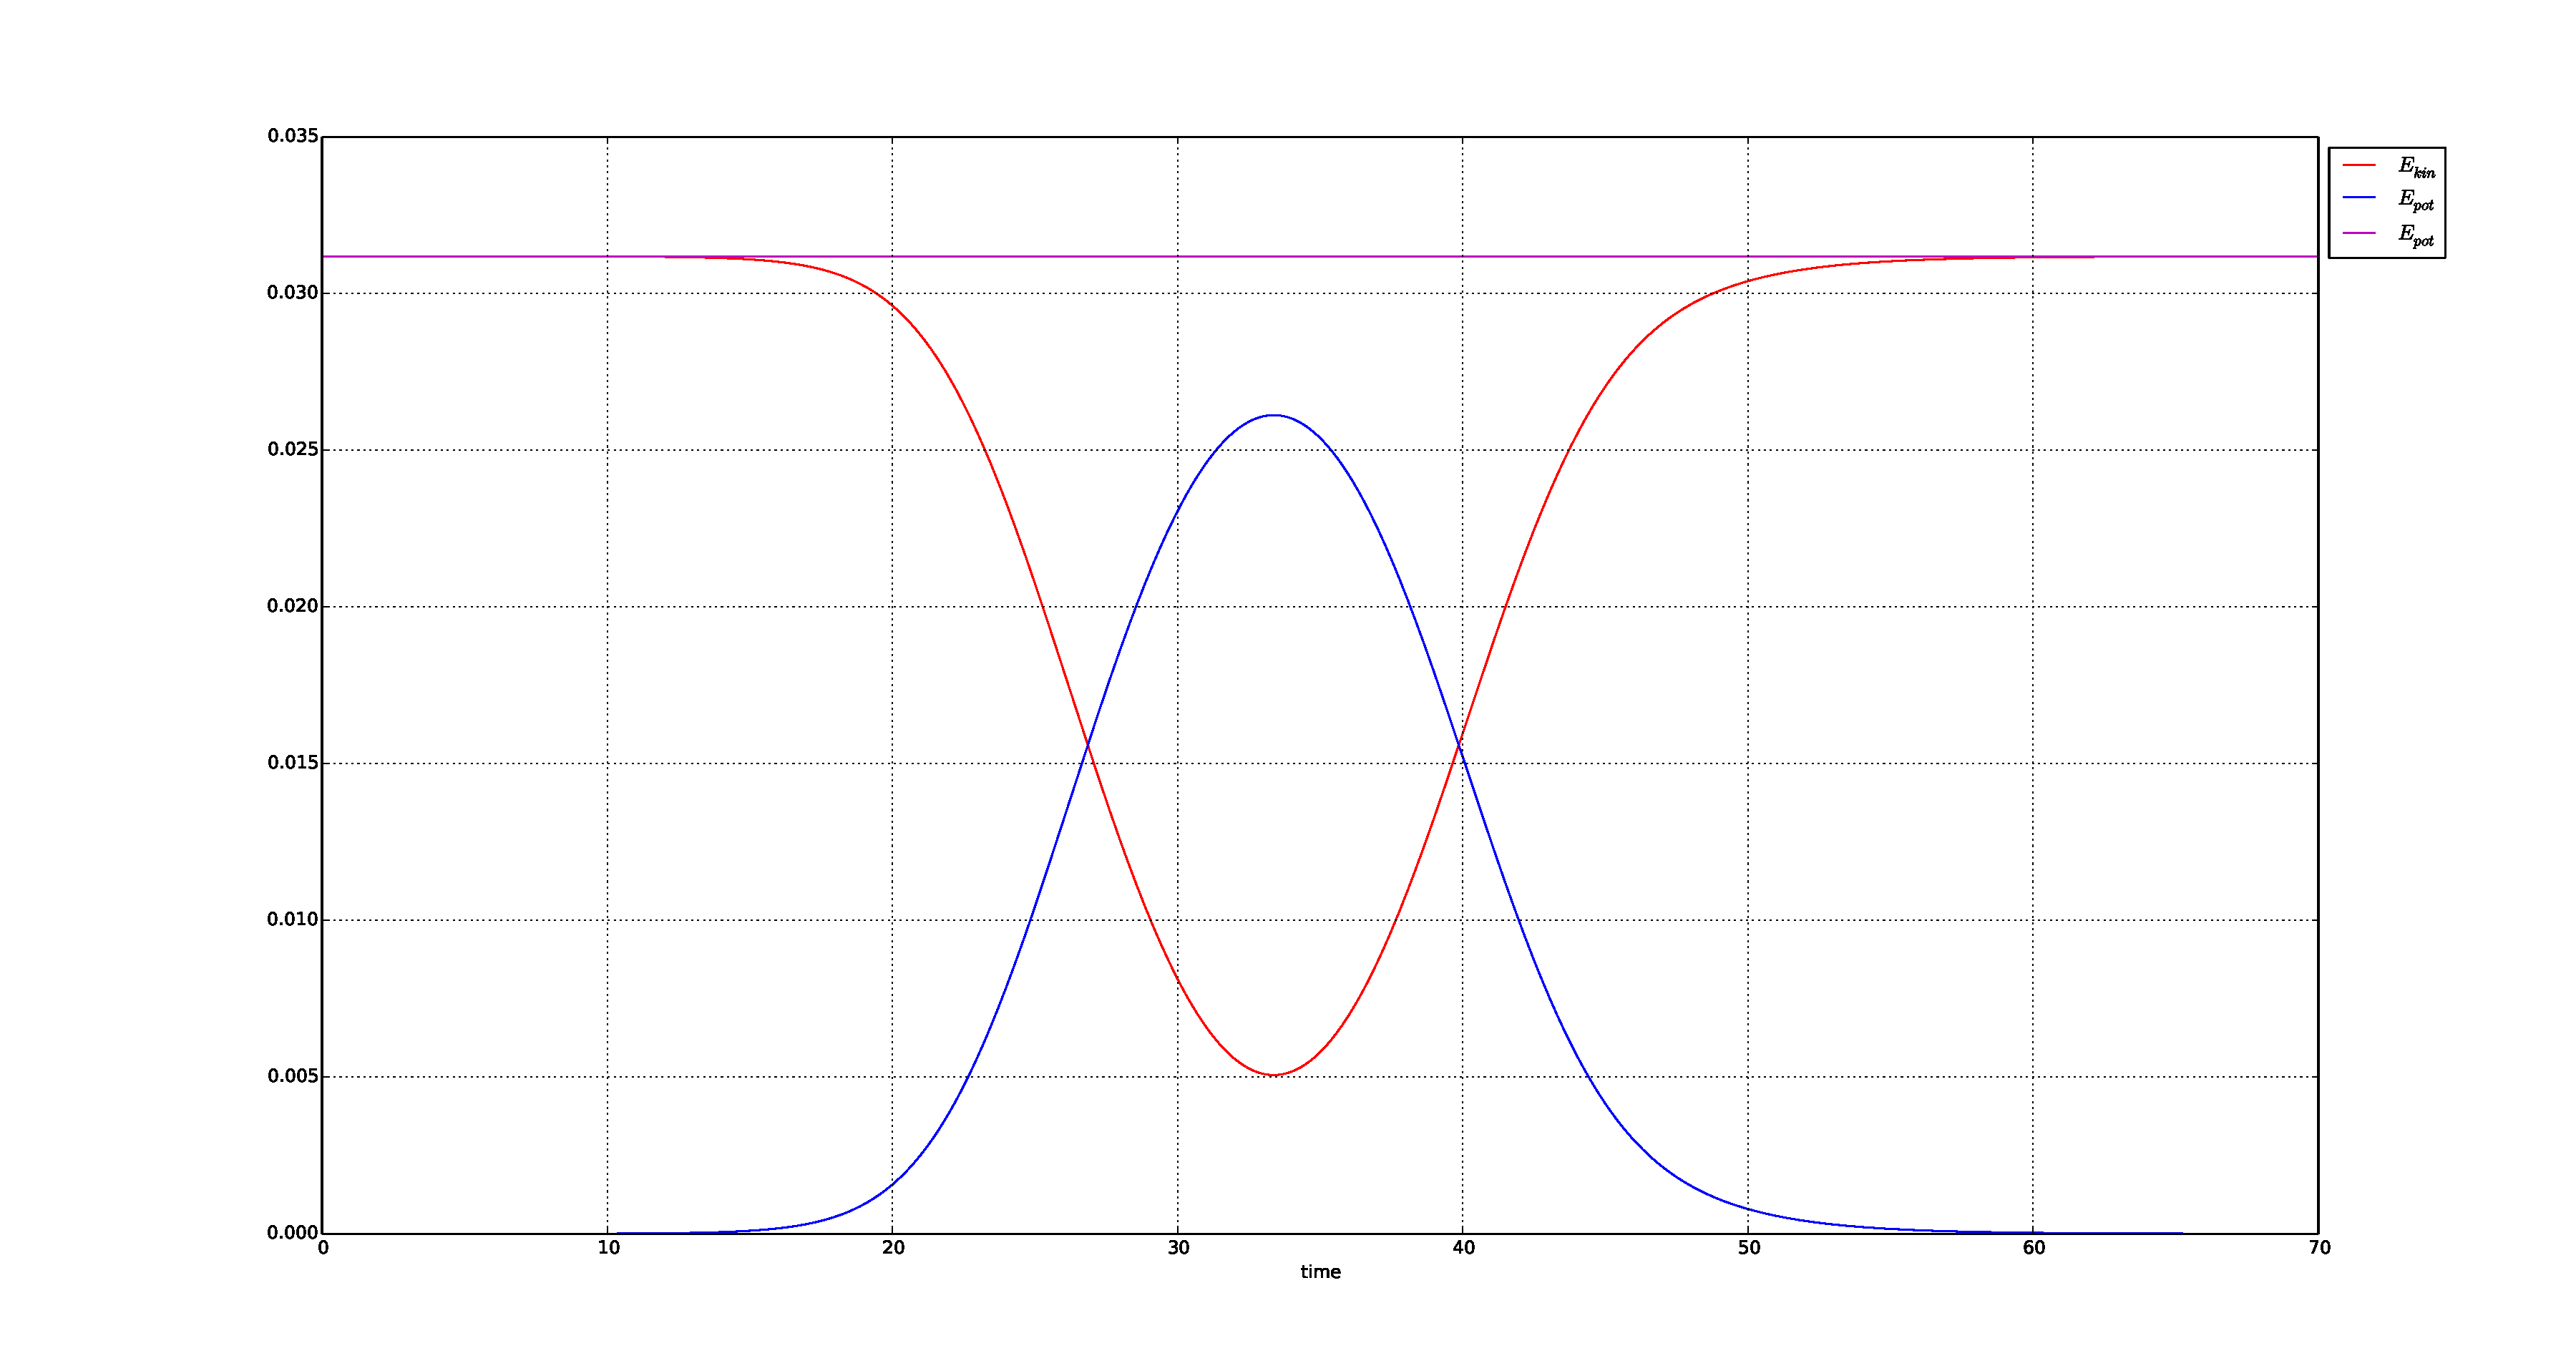
\includegraphics[width=\textwidth]{Figures/tunneling_energy.pdf}
\caption{Energies of the Tunneling Simulation}
\label{fig:tunneling_energy}
\end{figure}

\begin{figure}
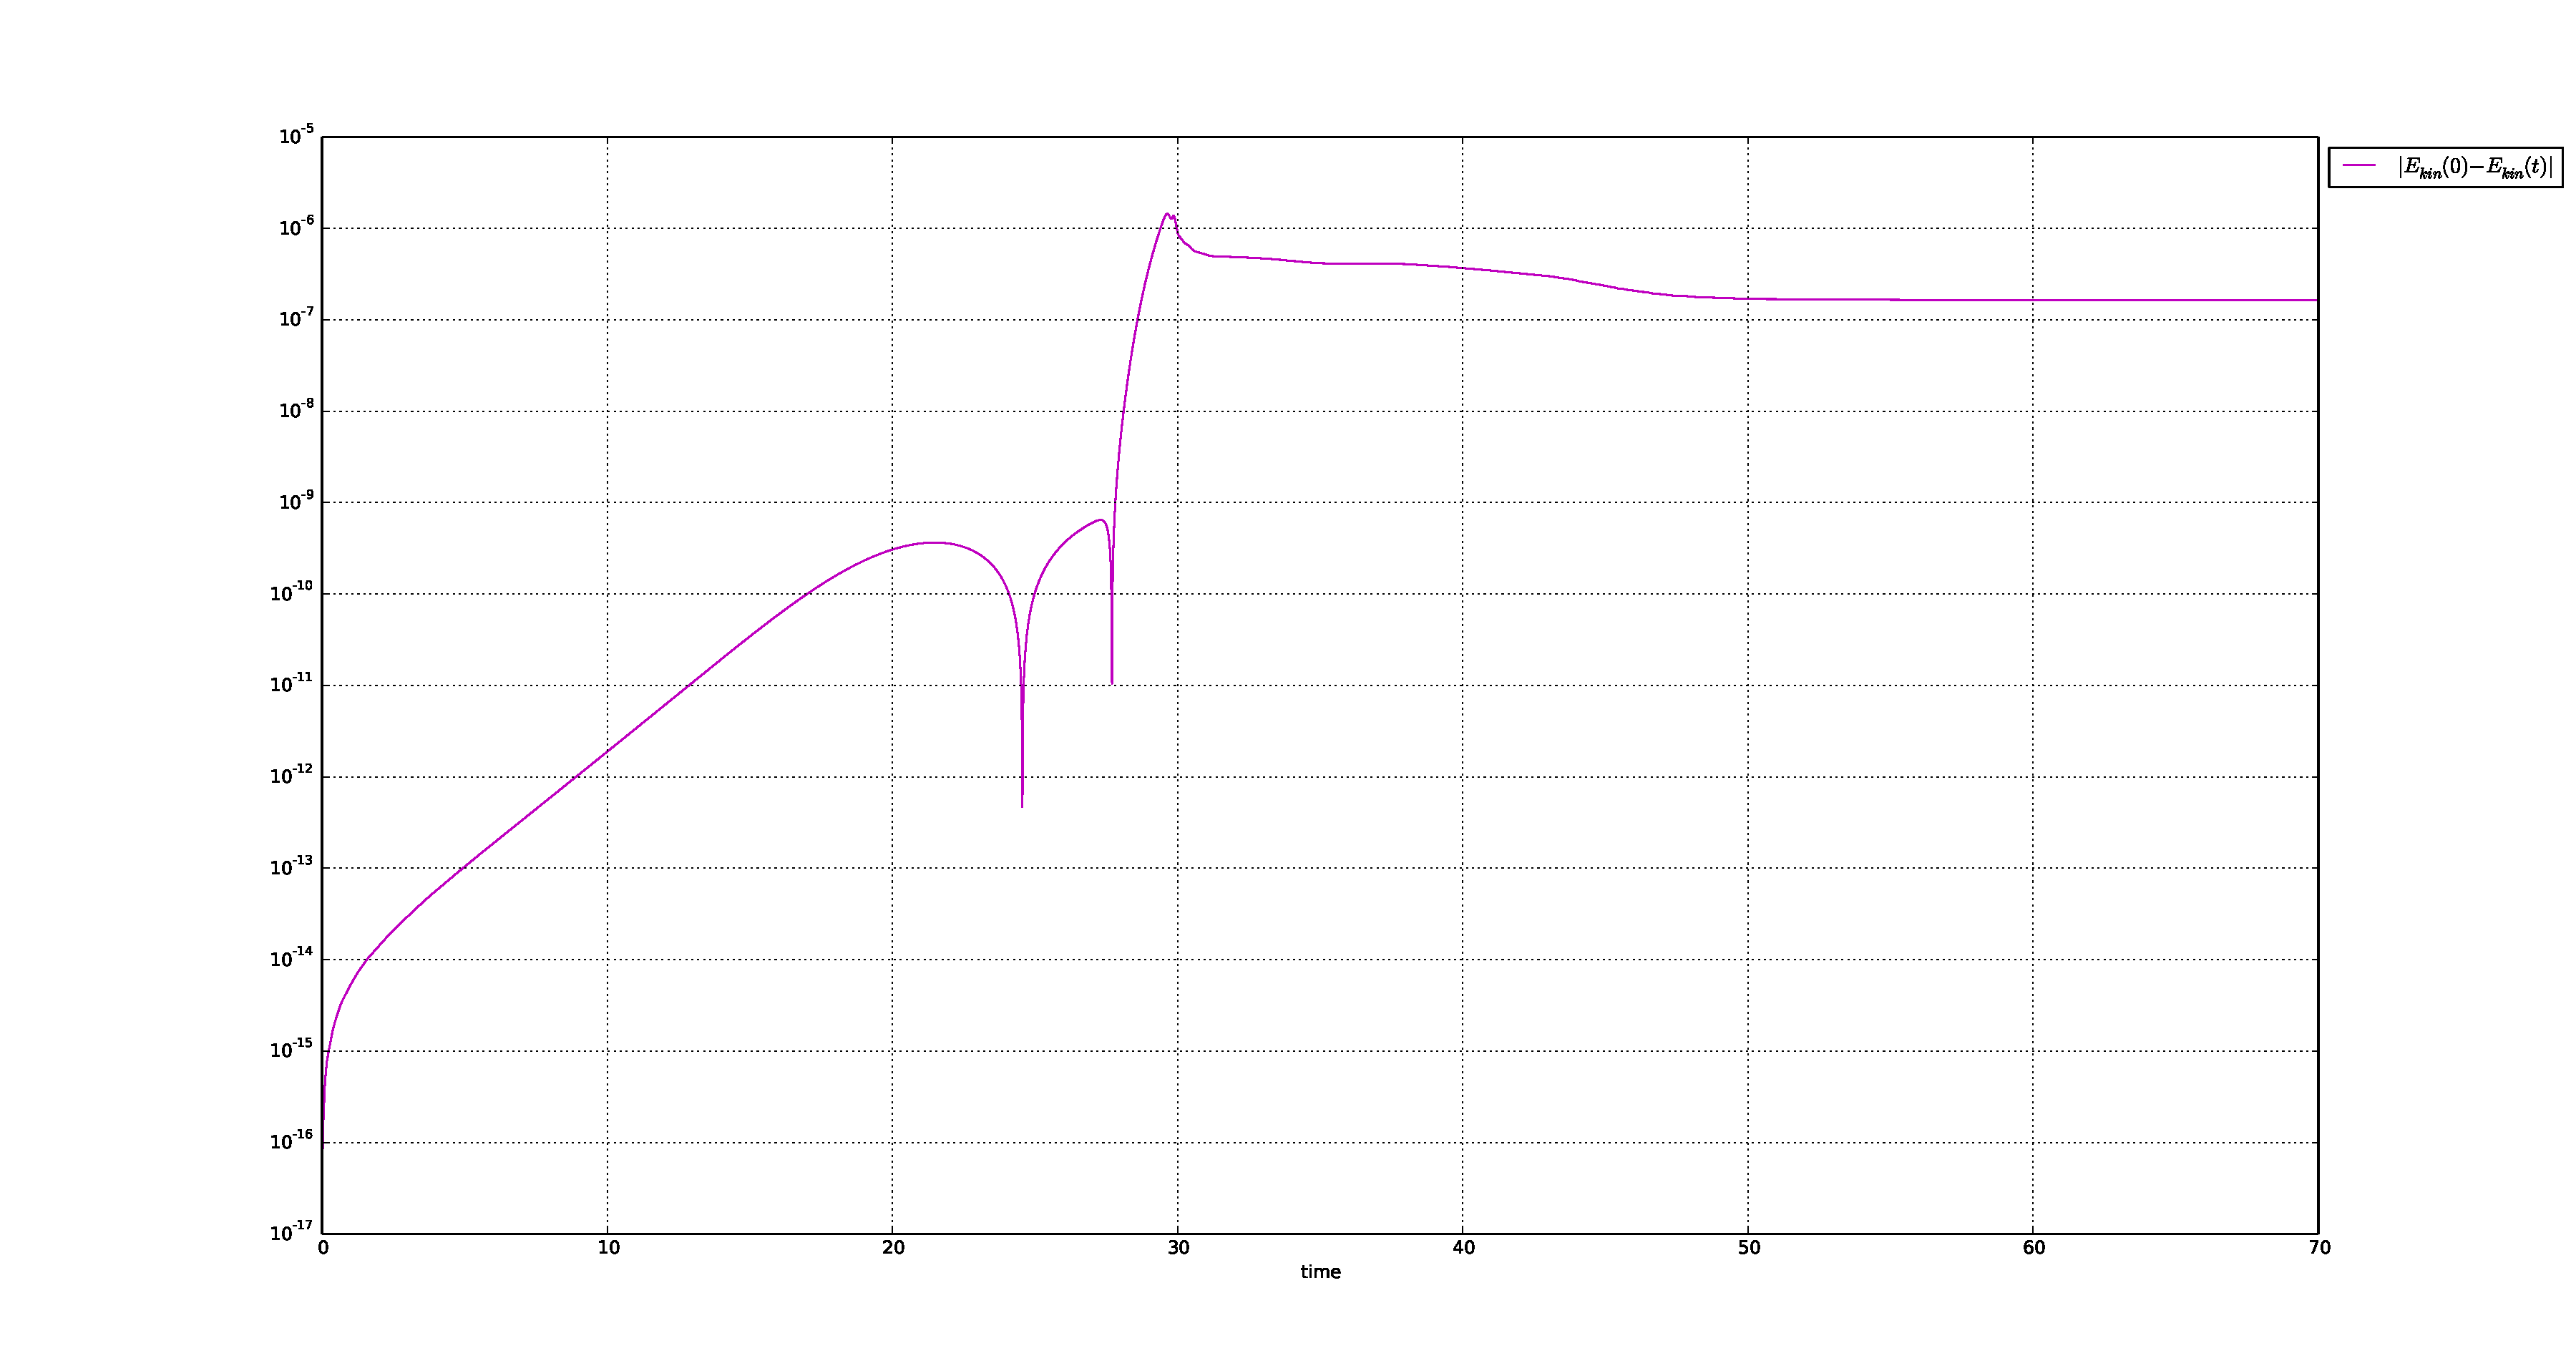
\includegraphics[width=\textwidth]{Figures/tunneling_drift.pdf}
\caption{Drift of Total Energy of the Tunneling Simulation}
\label{fig:tunneling_drift}
\end{figure} 	 	
\begin{figure}
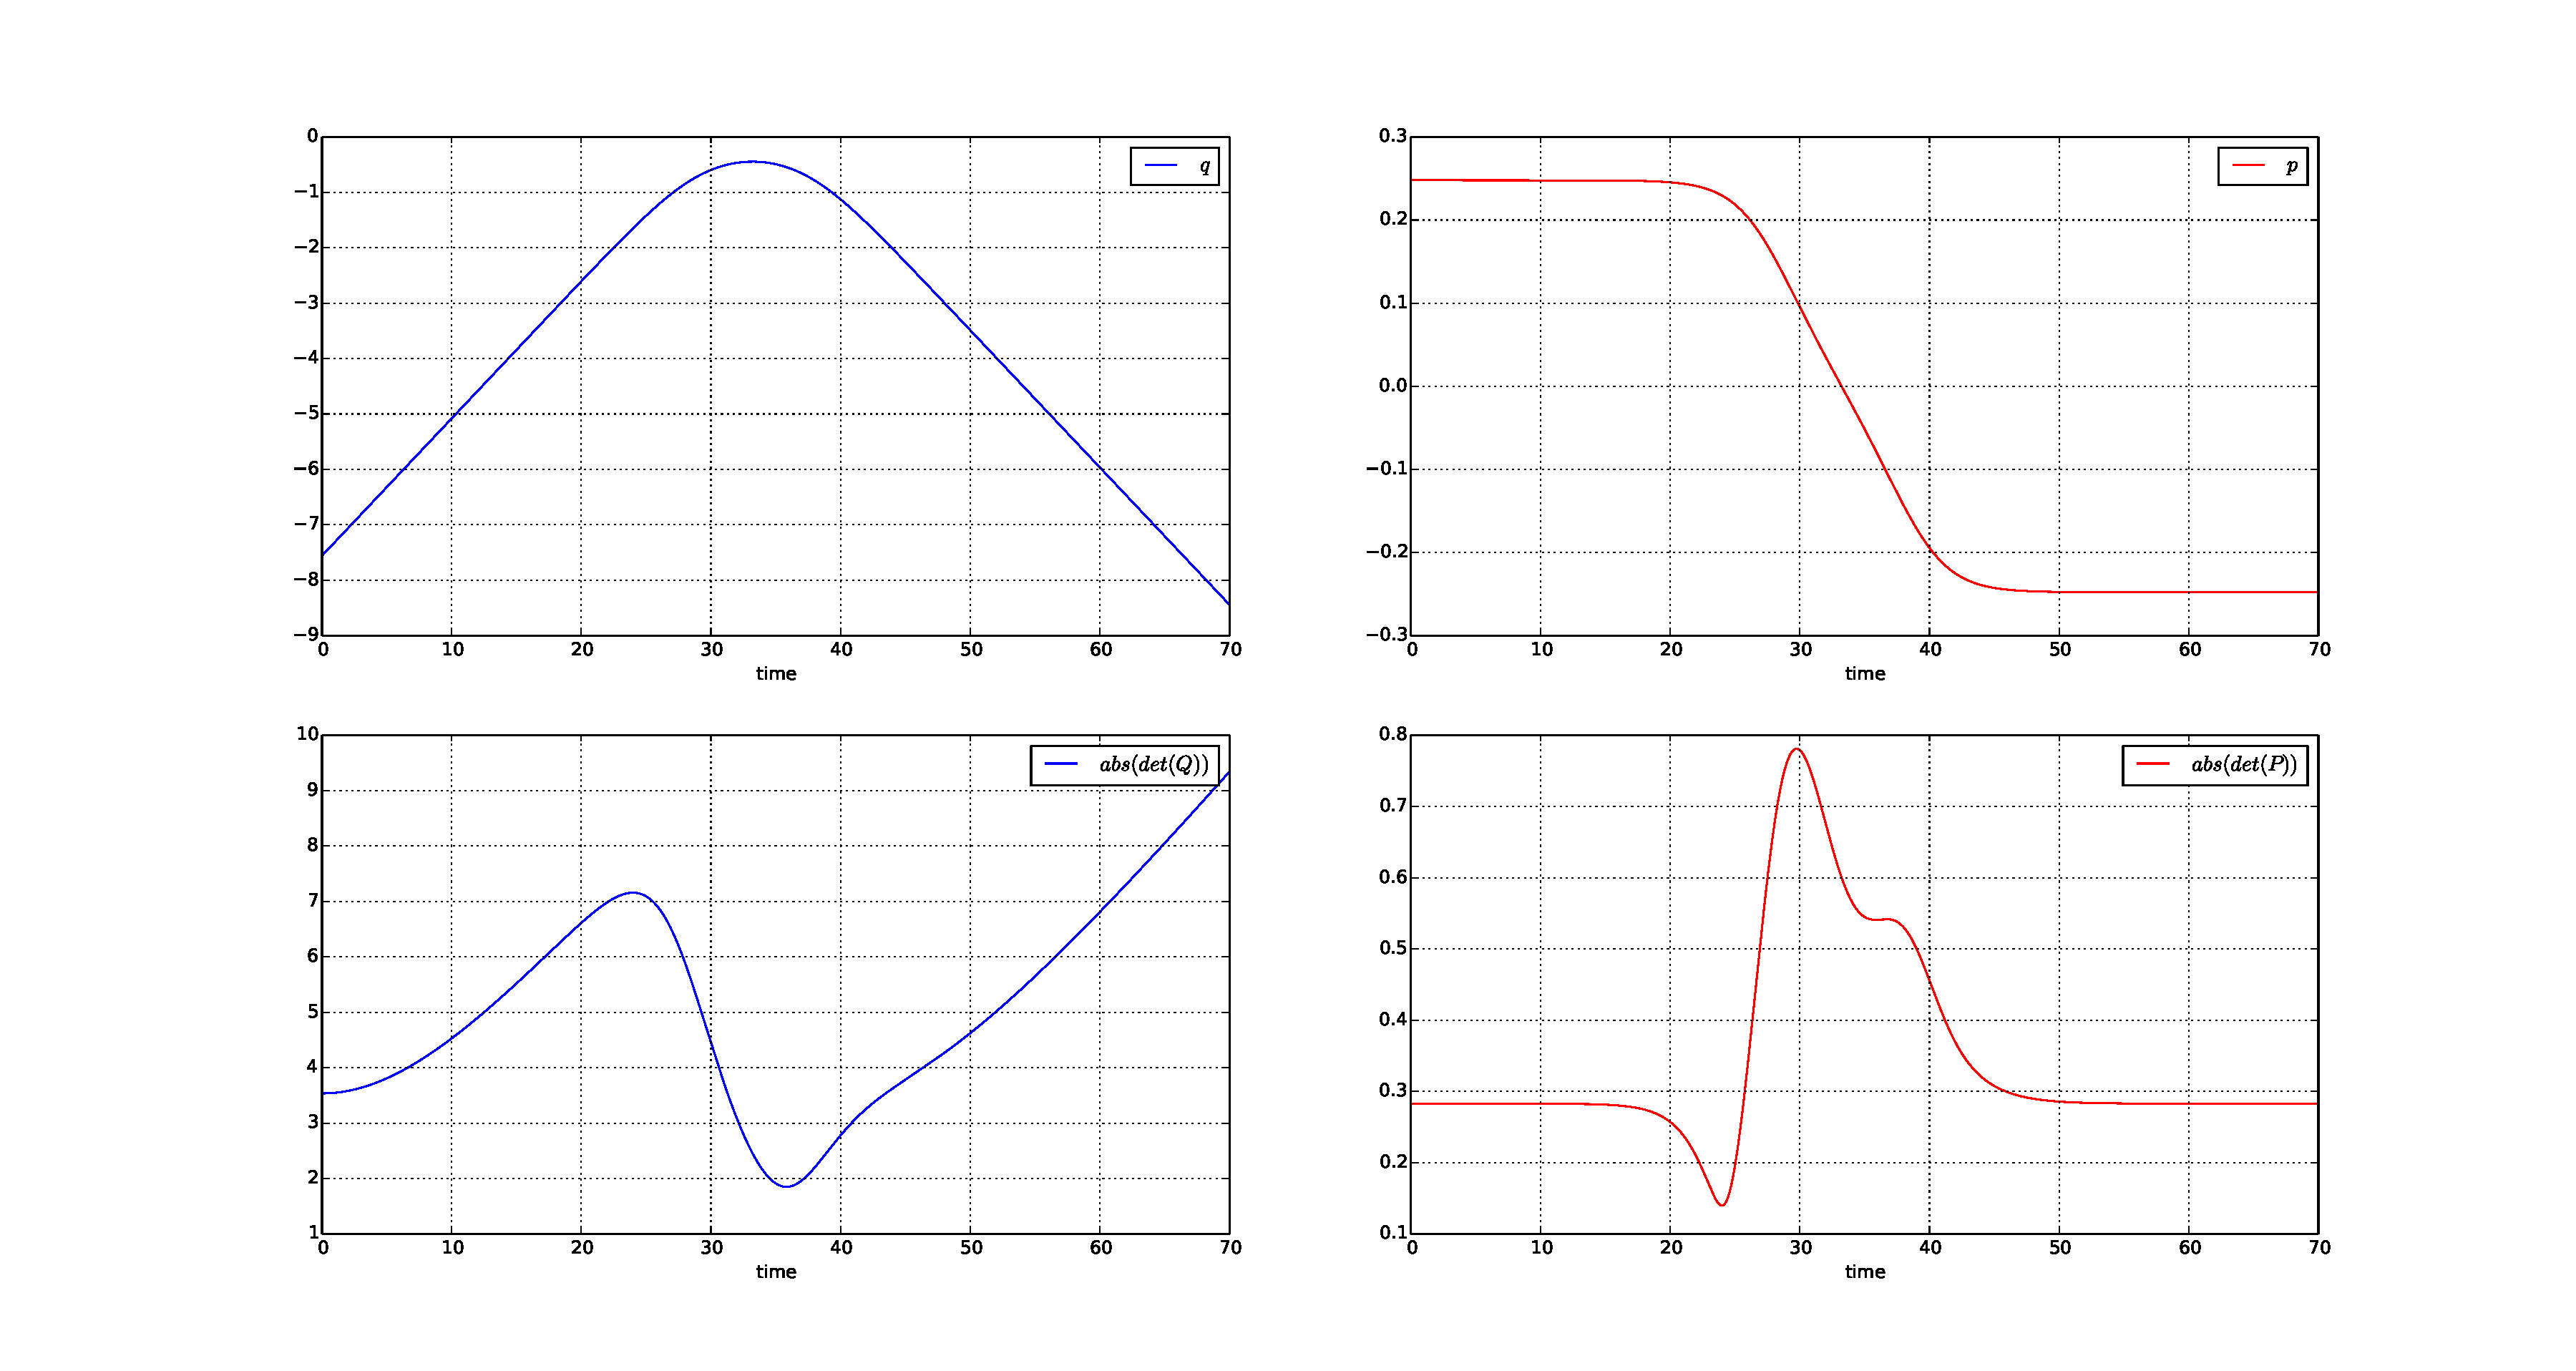
\includegraphics[width=\textwidth]{Figures/tunneling_params.pdf}
\caption{Position and Momentum Parameters}
\label{fig:tunneling_params}
\end{figure}
\begin{figure}
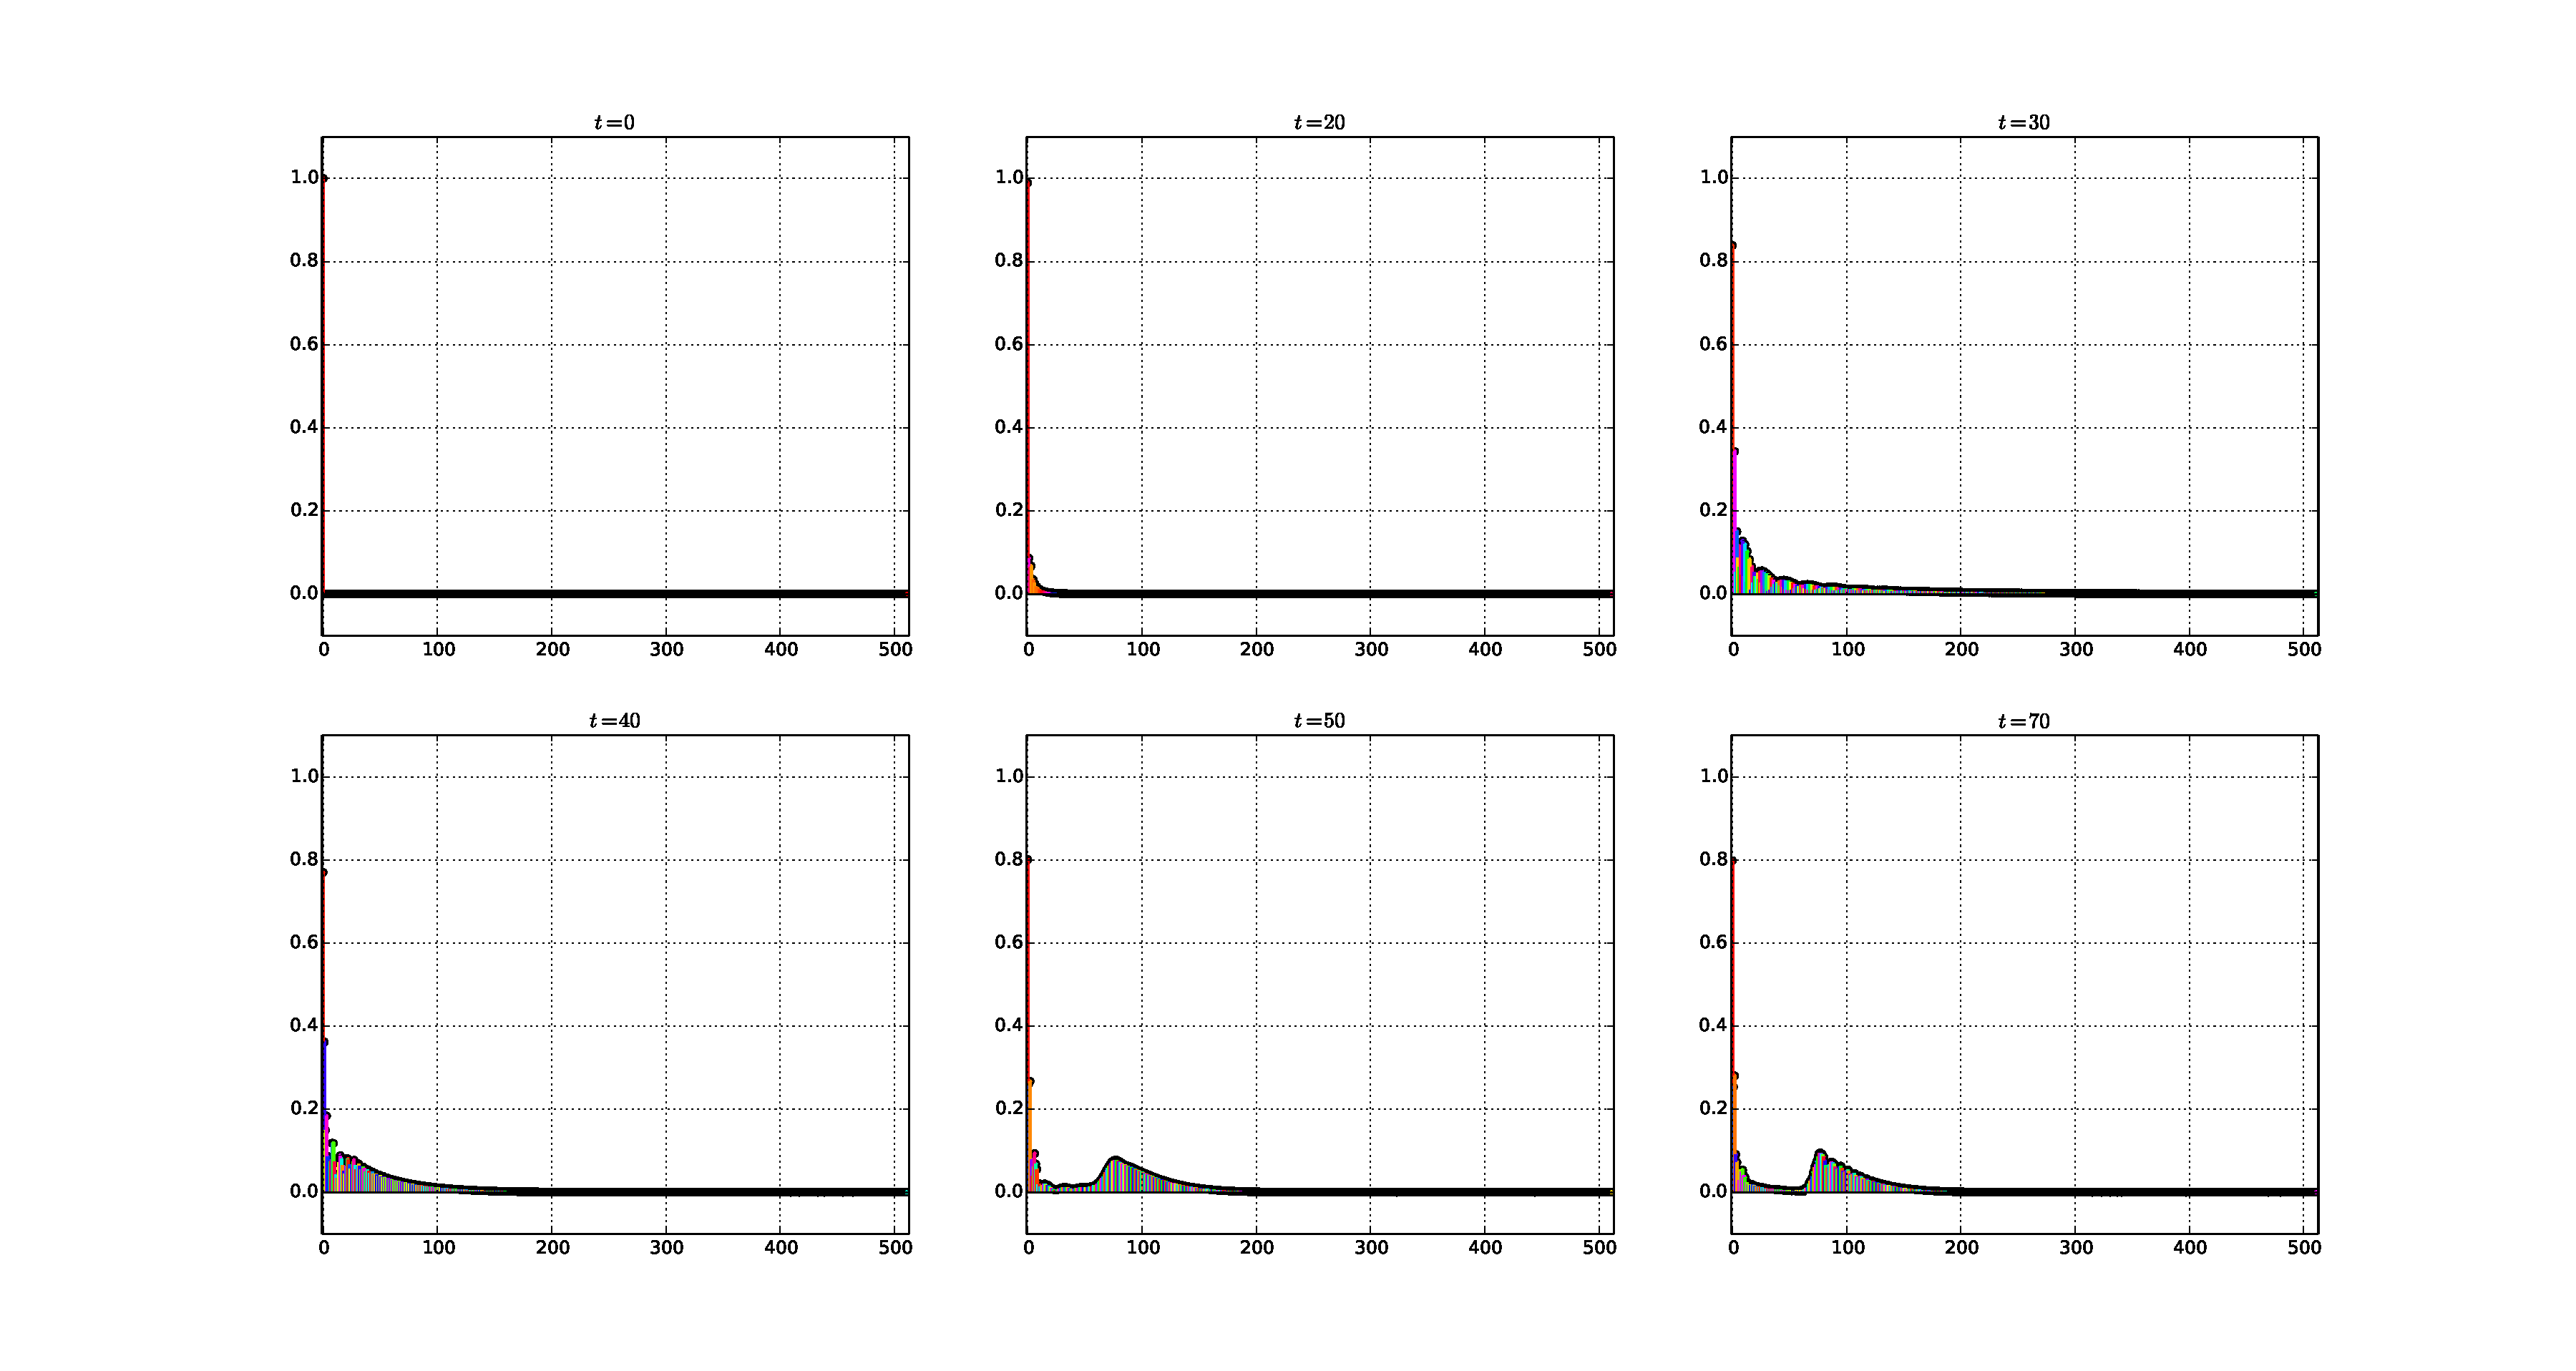
\includegraphics[width=\textwidth]{Figures/tunneling_coeffs.pdf}
\caption{Coefficients}
\label{fig:tunneling_coeffs}
\end{figure}

\begin{figure}
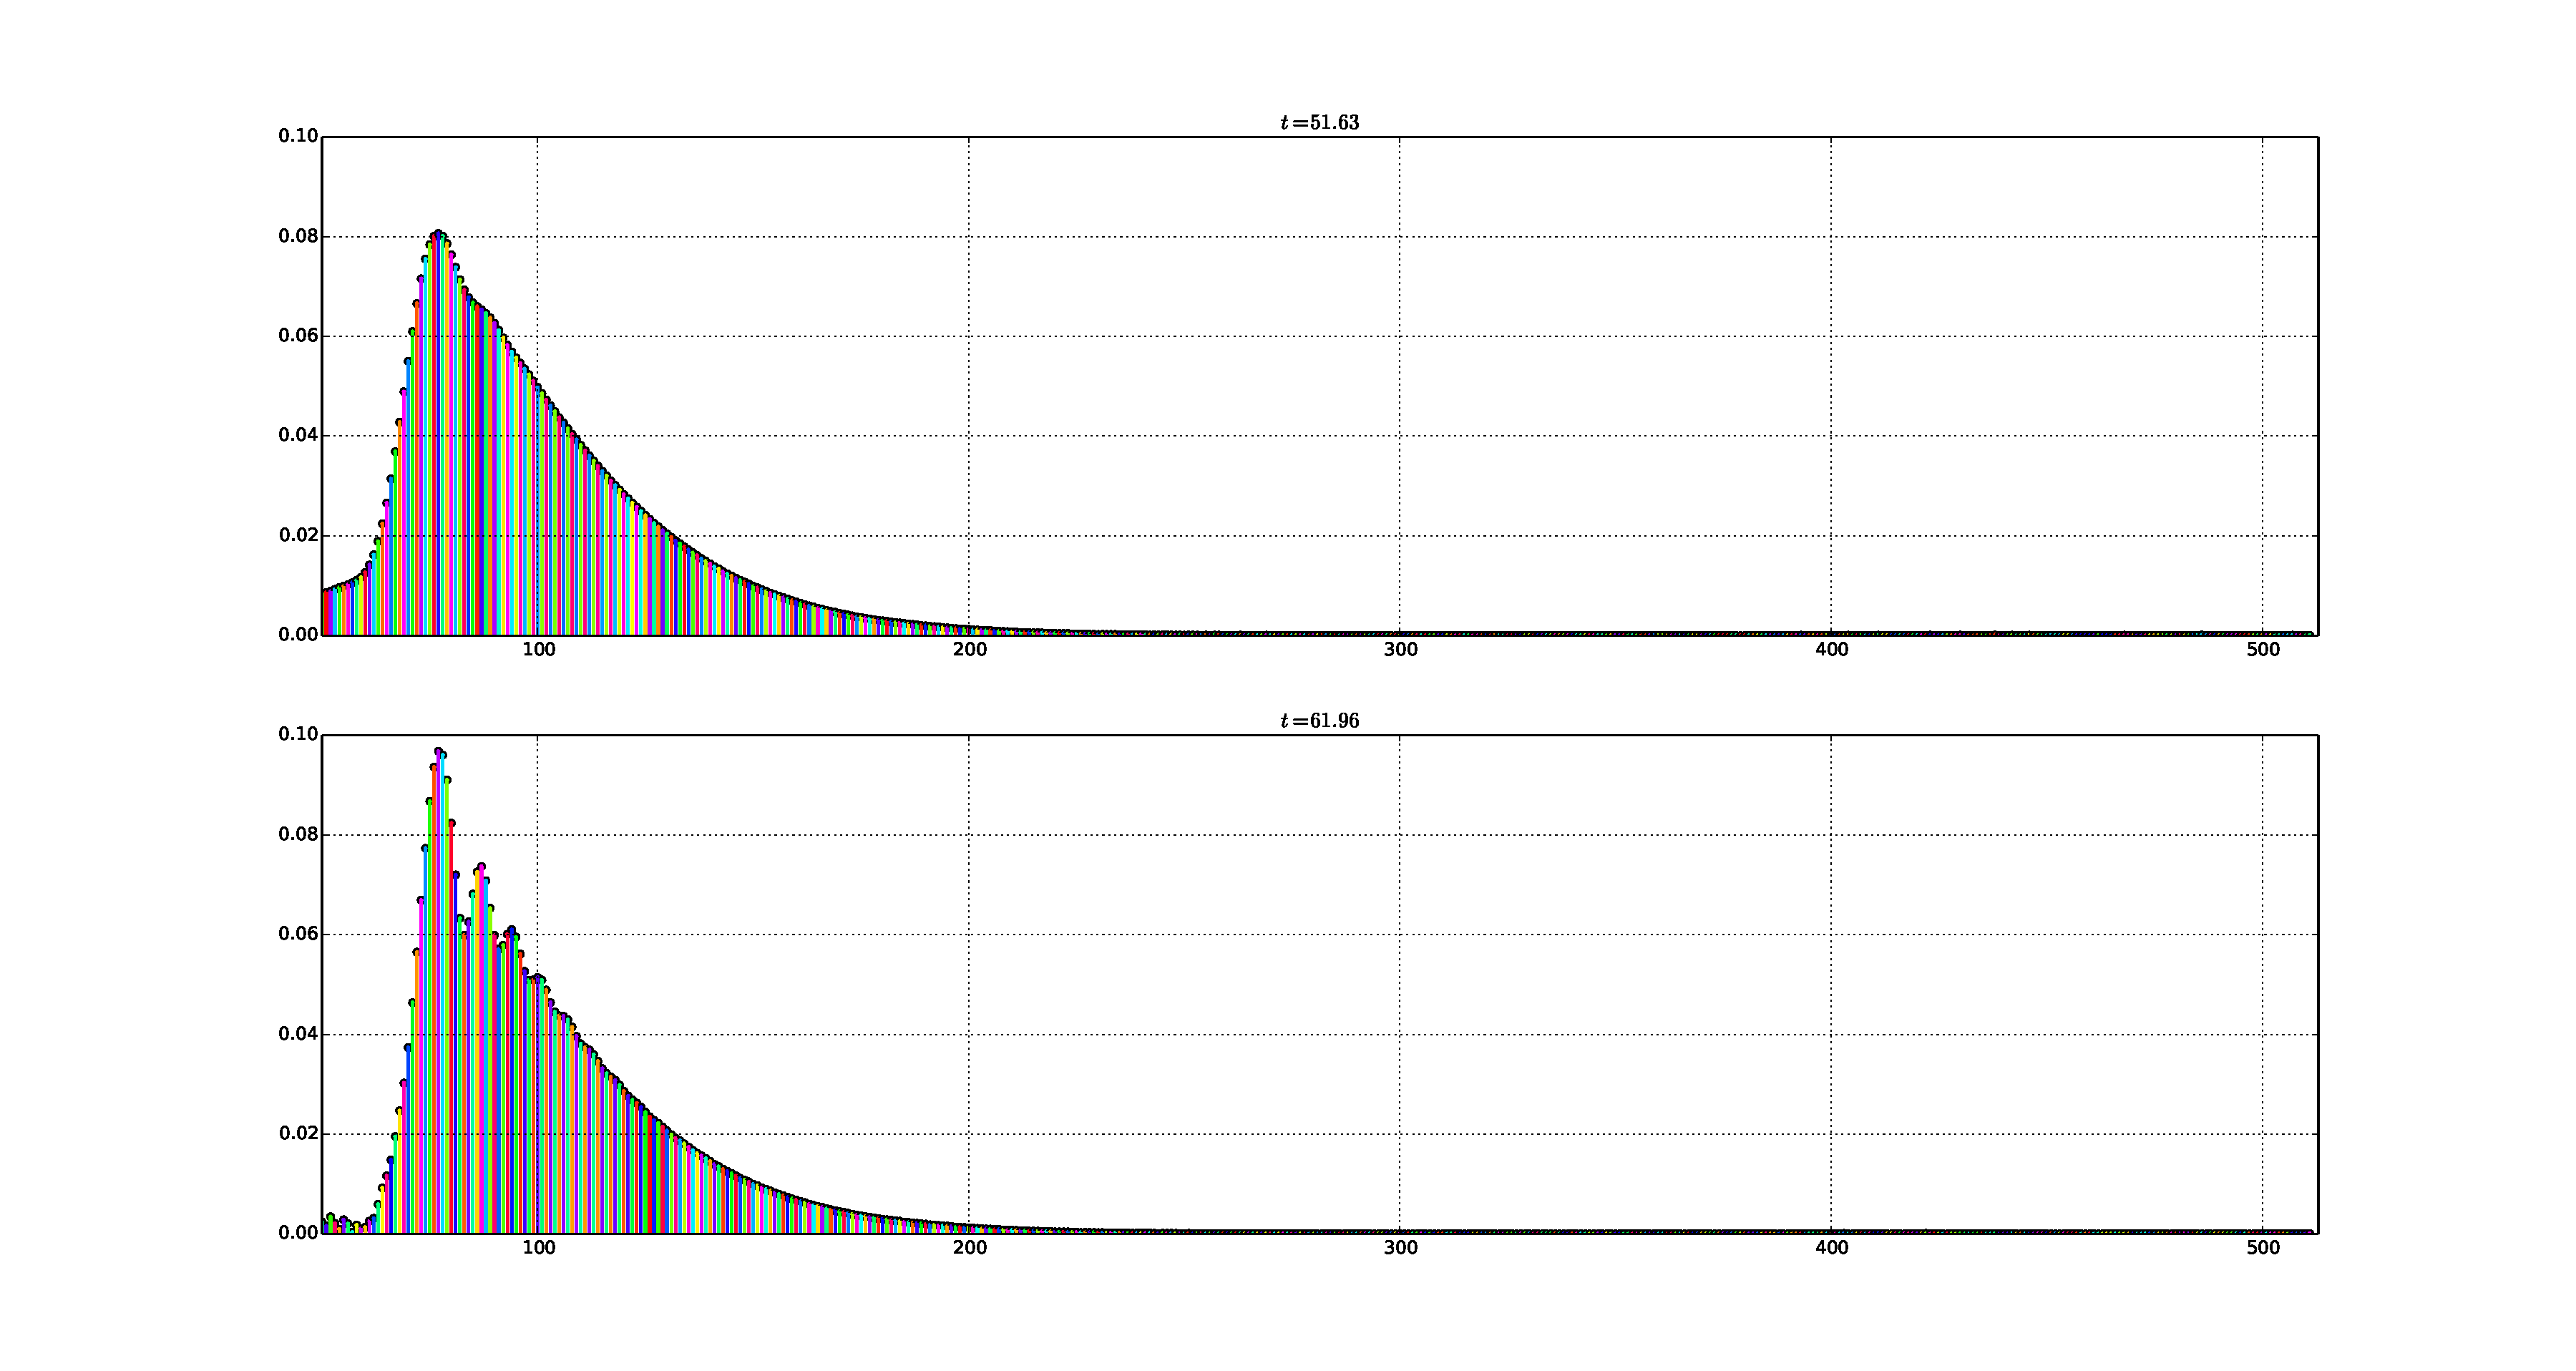
\includegraphics[width=\textwidth]{Figures/tunneling_coeffs_close.pdf}
\caption{close-up of Higher Order Coefficients}
\label{fig:tunneling_coeffs_close}
\end{figure}

\begin{figure}
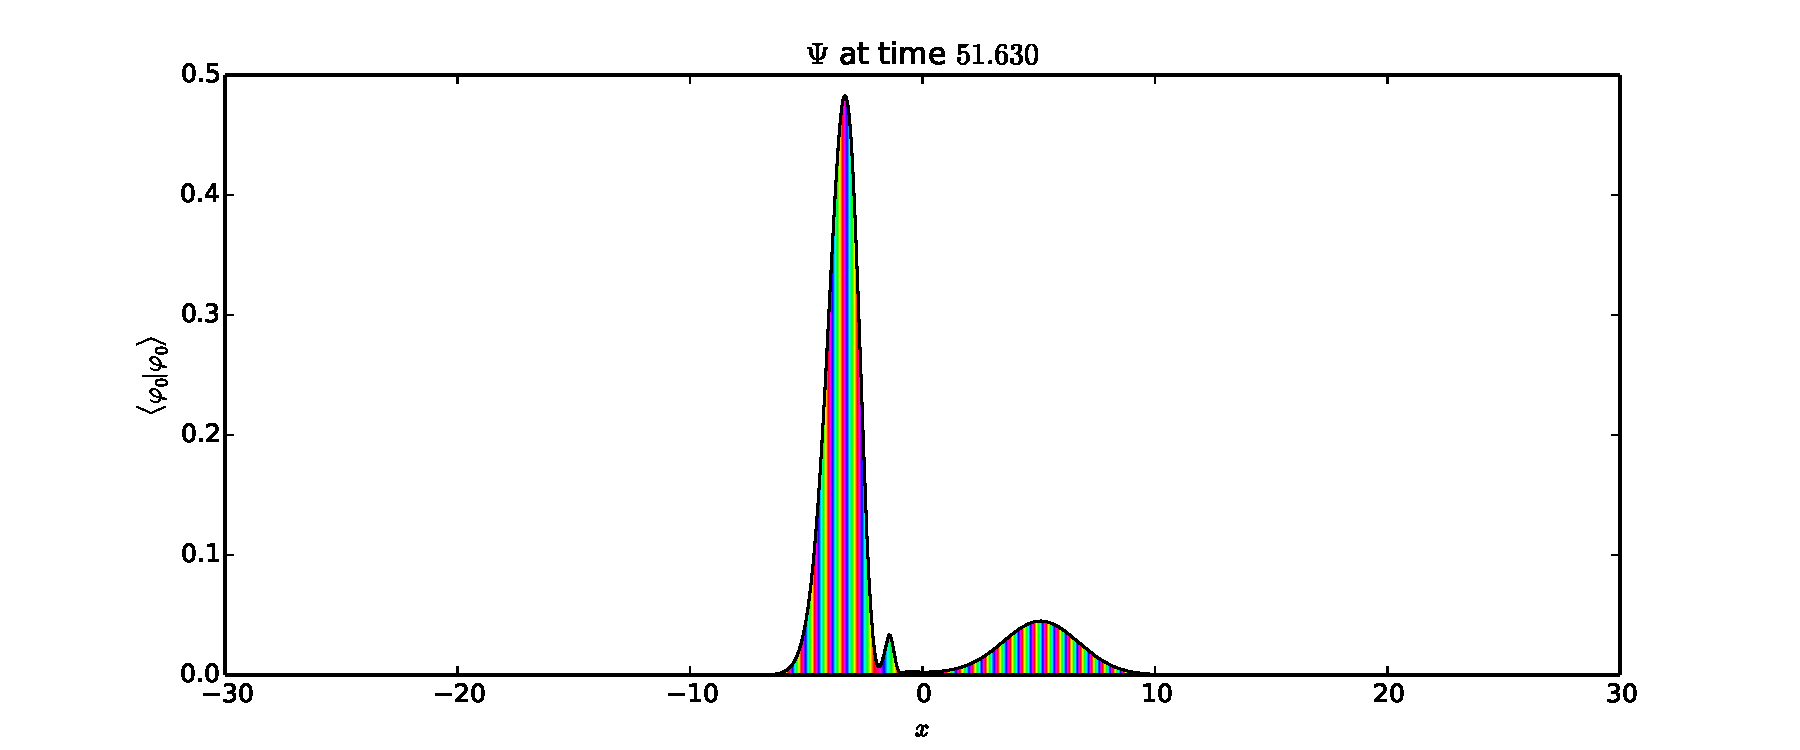
\includegraphics[width=\textwidth]{Figures/wavepacket_timestep_51_630.pdf}
\caption{$|u^2|$ at $t=51.63$}
\label{fig:wavepacket_at_51_63}
\end{figure}

\begin{figure}
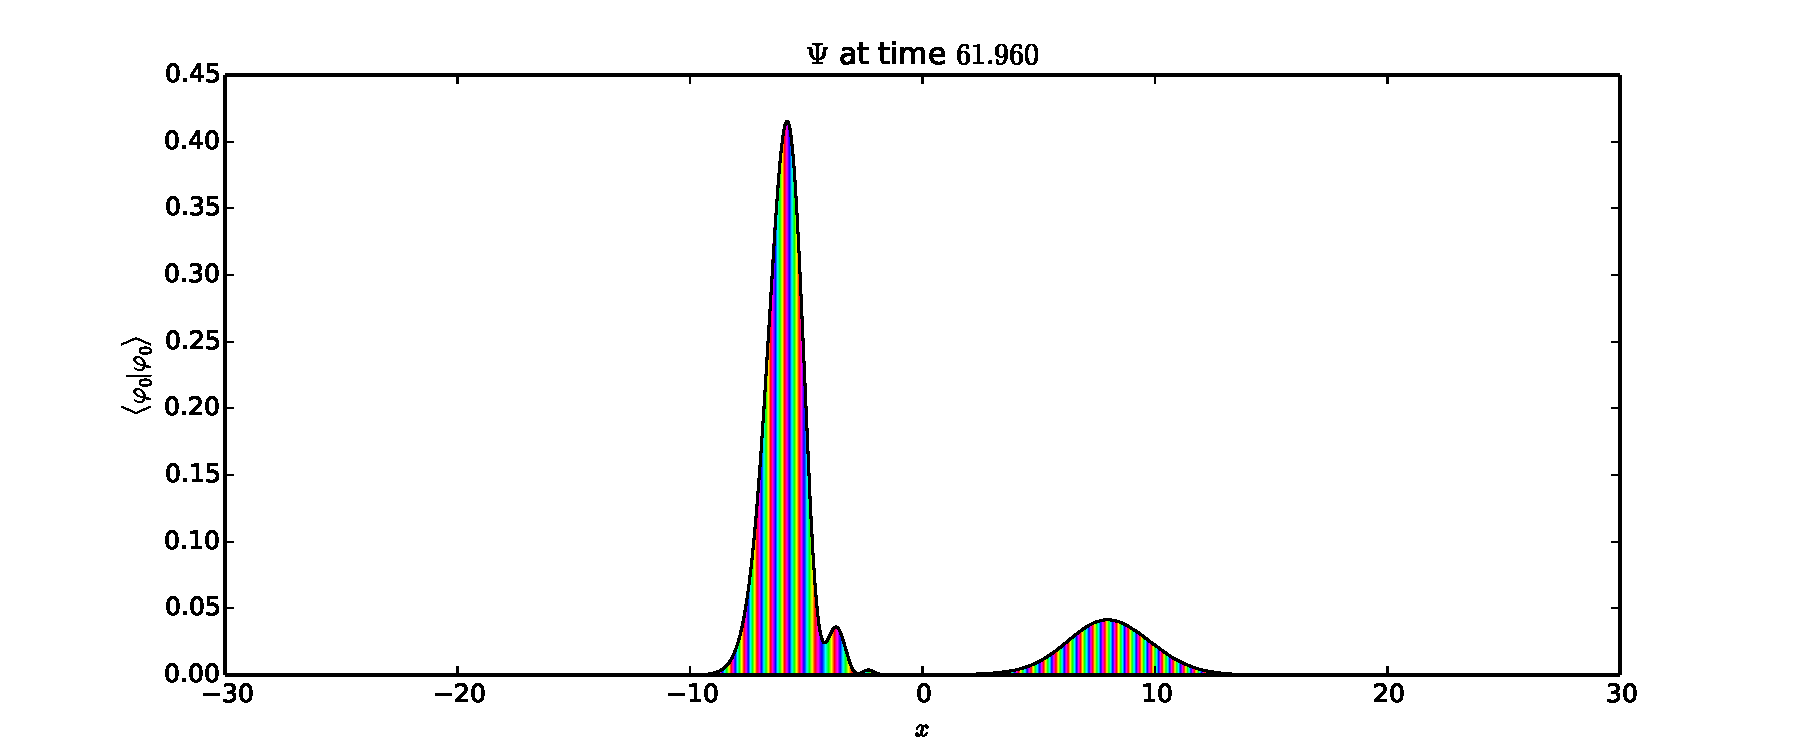
\includegraphics[width=\textwidth]{Figures/wavepacket_timestep_61_960.pdf}
\caption{$|u^2|$ at $t=61.96$}
\label{fig:wavepacket_at_61_96}
\end{figure}
\FloatBarrier
